\documentclass[11pt]{article}
\usepackage[utf8]{inputenc}
\usepackage{amssymb}
\usepackage{amsthm}
\usepackage{amsmath}
\usepackage{mathabx}
\usepackage{geometry}
\usepackage{breqn}
\usepackage{graphicx}
\usepackage{bbm}
\usepackage{tabularx}
\usepackage{adjustbox}
\usepackage{threeparttable}
\usepackage{mathtools}
\usepackage{float}
\usepackage{multirow}
\usepackage{mathrsfs}
%\usepackage{apacite}
\usepackage{caption}
\usepackage{subcaption}
\usepackage{booktabs}
\usepackage[table]{xcolor}
\usepackage{color,soul}
\usepackage{placeins}
\usepackage[english]{babel}
\usepackage{array}
\usepackage{textcomp}
\usepackage{eurosym}


\graphicspath{{Figures/}}

 \usepackage{epigraph}
    \renewcommand\textflush{flushright}

    \usepackage{etoolbox}
    \makeatletter
    \newlength\epitextskip
    \pretocmd{\@epitext}{\em}{}{}
    \apptocmd{\@epitext}{\em}{}{}
    \patchcmd{\epigraph}{\@epitext{#1}\\}{\@epitext{#1}\\[\epitextskip]}{}{}
    \makeatother

    \setlength\epigraphrule{0pt}
    \setlength\epitextskip{2ex}
    \setlength\epigraphwidth{.8\textwidth}


\usepackage{enumerate}
\numberwithin{equation}{section}
%\setlength\parindent{0pt}
\renewcommand{\qedsymbol}{$\blacksquare$}
%\selectlanguage{spanish}
\geometry{letterpaper, margin=1in}
%\pagestyle{headings}

\usepackage[style=apa, natbib=true, backend=biber, 
bibencoding=utf8,
maxbibnames=99,
sorting=nyt,
%maxcitenames=7,%modified
citetracker=true%added
]{biblatex}
\usepackage{csquotes}

\addbibresource{BID_Bib.bib}

\newcommand\nth{\textsuperscript{th}\xspace}
%\newcommand\st{\textsuperscript{st}\xspace}
\newcommand{\interior}[1]{%
  {\kern0pt#1}^{\mathrm{o}}%
}

\usepackage{ulem}
\usepackage{setspace}

\usepackage{blkarray}


\DeclareMathOperator*{\argmax}{arg\,max}
\DeclareMathOperator*{\argmin}{arg\,min}

\makeatletter
\newcommand{\vast}{\bBigg@{4}}
\newcommand{\Vast}{\bBigg@{5}}
\makeatother

\newtheorem{theorem}{Theorem}[section]
\newtheorem{corollary}{Corollary}[theorem]
\newtheorem{proposition}{Proposition}[section]
\newtheorem{lemma}{Lemma}[section]
%\theoremstyle{definition}
\newtheorem{definition}{Definition}
\theoremstyle{remark}
%\newtheorem*{remark}{Remark}

\normalem
\onehalfspacing
\geometry{left=1.0in,right=1.0in,top=1.0in,bottom=1.0in}

\interfootnotelinepenalty=10000

%Always Last

\usepackage[%
  colorlinks=true,%
  urlcolor=blue,%
  citecolor=.,
  linkcolor=.]{hyperref}

\AtEveryCitekey{\clearlist{publisher}}
\AtEveryBibitem{\clearlist{publisher}}



\begin{document}

\begin{titlepage}
\title{Estimation of the Marginal Cost of Health Produced by the Dominican Republic Healthcare System}
\author{Álvaro J. Riascos Villegas\thanks{Email: \href{mailto:alvaro.riascos@quantil.com.co}{alvaro.riascos@quantil.com.co}. We are grateful to Douglas Newball and Cristhian Acosta, who participated in early stages of this project. I would like to express my gratitude for the support and assistance in the preparation of this work to Yesenia Diaz Medina (Director of Health Insurance in Contributory Regimes and Plans - SISALRIL), Leticia Martínez (Director of Actuarial Studies - SISALRIL), Juan Ernesto Mercedes Ulloa (Statistical Data Analyst in the Department of Actuarial Analysis - SISALRIL), Dr. Yocastia De Jesús Arámboles (General Director of the Vice Ministry of Collective Health - Ministry of Public Health of the Dominican Republic), Dr. Clares Shayra Pérez (Director of Health Situation Analysis, Monitoring, and Evaluation of Results - Vice Ministry of Collective Health), Lic. Guillermina Rodríguez (Health Information Department - Ministry of Public Health), Engineer Engels Cruz (IT Support - Health Information Department of the Ministry of Public Health), Professor James Lomas (Department of Economics - University of York), Dr. Francesco Longo (Center for Health Economics - University of York), and Catalina Gutierrez (Senior Consultant in Social Protection, Labor Markets, and Health Economics - Inter-American Development Bank). The errors, opinions, methods, or results of this study do not bind or necessarily represent the views of any of the individuals or organizations mentioned and are the sole responsibility of the authors.} \\ University of the Andes and Quantil \and Santiago Torres \\ MIT %\and Douglas Newball \\ University of Southern California y Quantil \and Cristhian Acosta \\ Quantil
}
\date{\today}

\maketitle 
\begin{abstract}
This study uses quantitative techniques from the health economics literature for evaluating the cost-effectiveness of financing new technologies (including procedures and medications) that result in greater well-being and health for the country. Specifically, a methodology is developed to estimate the cost-effectiveness threshold (CET) for the public healthcare system of the Dominican Republic. Since the CET measures the level of healthcare expenditure estimated to be necessary to gain one quality-adjusted life year (QALY) or some analogous measure of health outcome, this value provides a criterion for determining whether the financing of a new technology is cost-effective. Given a budget constraint, if the cost per QALY of a new technology exceeds the CET, its adoption would yield health benefits inferior to the technologies it displaces. Using econometric techniques, this study estimates the expenditure elasticity of health outcomes with respect to healthcare spending at $-0.356$ (SE $= 0.114$). This estimate implies a CET for the Dominican Republic of 86,498 Dominican pesos (DOP), with confidence intervals of 40,832 DOP and 132,165 DOP, which is equivalent to $26\%$ of the per capita GDP in 2016 (330,949 Dominican pesos) with a confidence interval of $12.3\%$ to $39.9\%$ of per capita GDP, respectively. These results are robust to various econometric specifications and/or alternative measures of health outcomes.



\vspace{2mm}
\noindent\textbf{Keywords:} cost-effectiveness threshold; supply-side estimation; instrumental variables; Dominican Republic; health technology assessment; marginal cost of health \\

\bigskip
\end{abstract}
\setcounter{page}{0}
\thispagestyle{empty}
\end{titlepage}
%\pagebreak \newpage


\section{Introduction}

Health care systems in all countries are facing increasing health needs and, at the same time, limited health budgets. This has motivated governments to apply tools that promote the efficient use of resources. Economic evaluation has become an important factor in the decision-making process regarding financing new health technologies (procedures, medicines, among others), which improve wellbeing and health in the country. One of the tools used is the Cost-Effectiveness Threshold (CET). 
      According to \citet{Claxton2015}, the Cost-Effectiveness Threshold is defined as the level of health expenditure allocated to the health care system which is deemed to be necessary to gain one quality-adjusted life year (QALY) or an equivalent measurement for health outcomes.\footnote{YLL -- Years of life lost, AVAD -- disability-adjusted life years (Años de Vida Ajustados por Discapacidad), SEYLL -- Standard expected years of life lost.}  Therefore, given the budgetary restrictions of health expenditure, it is the opportunity cost – in terms of QALYs – to displace resources allocated initially to the Basic Health Plan (Plan Básico de Salud), towards the financing of new technologies (procedures, medicines, among others). The CET gives us an idea, whether a given health technology can be expensive for society or not. If the value of a new health technology is higher than the CET, its adoption would provide health benefits inferior to the technologies which would be displaced, which would lead to a net-loss in health. 
     This paper is a case study that uses data on life expectancy, mortality, and morbidity in the Dominican Republic, together with other sources of information, to estimate the cost-effectiveness threshold.


\citet{Culyer2016} offers an accessible explanation of this concept, emphasizing its particular value for developing countries: more severe resource constraints make it especially important to have a criterion for determining which procedures or medications are cost-effective and merit public funding. For example, ovarian cancer drugs such as Avastin, Taxol, and Paraplatin are not considered cost-effective in England, where the CET is estimated at \pounds12,936\footnote{Measured at constant 2008 prices. For further details, see \citet{Claxton2015}.} per QALY (quality-adjusted life year), yet these drugs carry an incremental cost-effectiveness ratio of \pounds144,000 per QALY according to the \textit{National Institute for Health and Care Excellence} (NICE) \parencite{Culyer2016}. By contrast, they fall within the range of medications considered cost-effective in Tanzania, where an indirect estimate of the Cost-Effectiveness Threshold stands at USD~\$7,300, equivalent to three times per capita income.\footnote{In the absence of a reliable CET estimate, the World Health Organization recommends using three times the country's per capita income as a reference threshold.} In a health system with a clear decision-making framework for coverage decisions, drugs of this type would clearly not be cost-effective. \\

Socially inefficient investments of this kind have driven a growing literature focused on the empirical estimation of the Cost-Effectiveness Threshold in other countries. Recent estimates place the CET between \euro{}21,000 and \euro{}24,000 for Spain, and at AUD~28,033 for Australia \parencite{Vallejo2018, Edney2018}. The research question motivating the present study is: what is the Cost-Effectiveness Threshold of the Dominican Republic's health care system? \\

The Dominican Republic currently lacks a formally adopted cost-effectiveness threshold for health technology assessment decisions under the Plan Básico de Salud. In the absence of a local estimate, decision-makers have relied on the WHO heuristic of one to three times per capita GDP as an informal reference. Producing a domestically grounded empirical estimate is therefore the central objective of this study.

The document is structured in the following way: after the introduction, the following section surveys the literature on the empirical estimation of cost-effectiveness thresholds. The chapter on data then describes the data related to the Dominican Republic used in this study. The following section on methodology outlines the calculation of the result variable in health, the estimation method of the elasticity of demand, as well as the calculation of the Cost-Effectiveness Threshold. The following section presents the results, and the concluding section draws the main conclusions and directions for future research.

\section{Literature Review}

The cost-effectiveness threshold (CET) specifies the maximum expenditure per unit of health gain that a health system should be willing to incur when operating under a fixed budget constraint. Two conceptually distinct approaches have been proposed to identify this value. The demand-side approach equates the threshold to the monetary value that individuals or society place on health gains, estimated through willingness-to-pay methods \parencite{Pandey2018}. The supply-side approach defines the threshold as the health opportunity cost of additional expenditure: the value of health foregone elsewhere in the system when resources are committed to a new technology \parencite{Culyer2016}. For decisions governed by fixed budgets, where new expenditure necessarily displaces existing care, the supply-side threshold---the cost of generating health within the current system---is the appropriate reference \parencite{Claxton2015}. This distinction is not semantic. Using a demand-side threshold in a fixed-budget setting implies adopting technologies that displace more health than they produce, reducing population health overall. The literature reviewed here concerns the supply-side approach and its empirical estimation.

The methodological framework for estimating the supply-side CET from within-country data was established by \citet{Claxton2015}. Their study estimated the marginal cost per quality-adjusted life year (QALY) produced by the English National Health Service (NHS) using data on 23 programme budget categories (PBCs) across 152 Primary Care Trusts (PCTs). For each disease area with a measurable mortality rate, the study estimated a two-stage least squares (2SLS) regression of years of life lost (YLL) on programme expenditure, using socioeconomic characteristics constructed from the Department of Health's resource allocation formula as instruments to address the endogeneity of expenditure. The disease-specific expenditure elasticities were then combined with information on the survival and morbidity burden of each disease to calculate the marginal cost per QALY produced. The central estimate was \pounds12,936 per QALY (2008/9 data), substantially below the \pounds20,000--\pounds30,000 range applied by the National Institute for Health and Care Excellence (NICE) as an acceptance threshold for new health technologies. This gap implies that technologies approved by NICE under the prevailing threshold systematically displace more NHS health than they generate, yielding a net health loss to the population. The identification structure of \citet{Claxton2015}---cross-sectional variation in expenditure and outcomes across subnational health units, instrumented to isolate exogenous spending shifts---is the identification structure adopted in the present study. The Dominican Republic's public health system allocates expenditure across municipalities and disease groups in a structure directly analogous to the English PCT-by-PBC panel, and this study estimates 2SLS regressions of disability-adjusted health outcomes on per capita health expenditure within disease-group-by-municipality cells.

\citet{Martin2021} updated and extended the Claxton approach by estimating annual outcome elasticities for ten disease areas from 2003/04 to 2012/13, using instruments derived from the NHS resource allocation formula (the ``funding rule''). The funding-rule variables---an input price index, an age-cost index, and the distance between each PCT's actual budget and its formula-calculated target---reflect administrative decisions in the allocation formula that are unrelated to local mortality patterns, satisfying the exclusion restriction on stronger grounds than the socioeconomic instruments used by \citet{Claxton2015}. The estimated annual marginal cost per QALY ranged from \pounds5,000 to \pounds10,000 over the study period, lower than the Claxton central estimate and consistent with a fall in the real marginal productivity of NHS expenditure as health budgets increased substantially after 2000. The consistency of results across two different IV strategies---funding-rule instruments and socioeconomic instruments---supports the robustness of the elasticity approach. The present study follows this robustness discipline by estimating the CET under four distinct IV strategies---contiguous municipalities, five nearest neighbors, ten nearest neighbors, and inverse-distance weighting---and testing instrument validity using the $C$-statistic of \citet{K.Newey1985}.

The methodology was subsequently applied to Spain and Australia. \citet{Vallejo2018} constructed a panel of 17 Spanish autonomous communities over 2008--2012, a period in which aggregate public health expenditure fell by approximately 10 percent as a consequence of fiscal consolidation. Using quality-adjusted life expectancy as the health outcome and the share of total public expenditure allocated to health as an instrument, they estimated a spending elasticity of 0.07, which implies a CET of \euro21,000--\euro24,000 per QALY, below the \euro30,000 figure commonly cited in Spain without empirical grounding. The austerity-driven cross-regional variation in health spending in Spain is conceptually comparable to the cross-municipal variation in the Dominican Republic's health budget, which reflects national-level allocation decisions transmitted asymmetrically across territories. \citet{Edney2018} applied the approach to Australia using cross-sectional data for 2011/12 across Statistical Local Areas. The study estimated both the mortality-related and the morbidity-related QALY effects separately, with the morbidity component derived directly from longitudinal health-related quality-of-life survey data rather than from a proportionality assumption applied to the mortality effect. The base-case CET was AUD~28,033 per QALY gained (95\% CI: AUD~20,758--37,667), below the AUD~40,000--60,000 range implicitly used by the Pharmaceutical Benefits Advisory Committee. The present study uses the AVAD (disability-adjusted life years incorporating both mortality and morbidity burden at the disease-group level) as the primary health outcome, which reduces dependence on the proportionality assumption that characterizes mortality-only approaches.

By 2022, within-country empirical estimates had been produced for seven countries across eight studies: England, Spain, Australia, the Netherlands (two studies with different methods), Sweden, South Africa, and China. \citet{Edney2022} reviewed these studies to document shared methodological choices and divergent decisions that affect the resulting estimates. The review identified endogeneity handling (panel fixed effects versus instrumental variables), measurement of health spending, level of disease aggregation, treatment of lagged expenditure effects, use of analytical population weights, and extrapolation from mortality to morbidity-adjusted outcomes as the primary sources of cross-country variation in results. The paper found that estimates based on contemporaneous spending and mortality may underestimate the long-run marginal productivity of expenditure, because the effects of past spending on current health are not captured. It recommended that future country estimates present both weighted and unweighted regressions, report tests of IV relevance and validity, and conduct sensitivity analyses across alternative specifications. The present study follows each of these practices: regressions are population-weighted (as in \citet{Claxton2015}), the Kleibergen-Paap $F$-statistic is reported for all specifications, instrument validity is assessed using the $C$-statistic, and the four IV strategies provide the primary robustness analysis.

Two additional papers address the challenge of providing threshold guidance for countries that lack the administrative data required for within-country estimation. \citet{Woods2016} extended the Claxton estimate to a wide range of countries by applying income elasticities of the value of a statistical life to the UK central estimate, on the assumption that the income elasticity of health opportunity costs tracks the income elasticity of the demand for health. Under an income elasticity of 1.5---the preferred estimate in the literature reviewed by the authors---countries at income levels comparable to the Dominican Republic face CETs in the range of 10--50 percent of GDP per capita, well below the World Health Organization's heuristic of 1--3 times GDP per capita. \citet{PichonRiviere2023} estimated thresholds for 174 countries from historical data on health expenditure per capita and life expectancy growth, deriving the CET consistent with keeping the rate of health spending growth within the secular trend observed for countries at each income level. Their results show that the CET is below one times GDP per capita in 97 percent of the 174 countries analyzed; for upper-middle-income countries---the World Bank income group that includes the Dominican Republic---31 percent have a threshold below 0.5 times GDP per capita. The present study's estimate of 86,498 Dominican pesos, equal to approximately 26 percent of 2016 per capita GDP, falls in this range and is therefore consistent with both frameworks' projections for a country at the Dominican Republic's income level.

Progress toward within-country estimation in Latin America has been concentrated in Colombia. \citet{Espinosa2021} estimated the supply-side CET for Colombia using administrative data from health insurers operating under the managed-competition structure of the Sistema General de Seguridad Social en Salud (SGSSS) for the period 2013--2017. The analysis constructed a panel of cells defined by insurer, geographic region, ICD-10 disease chapter, and year; endogeneity was addressed through two instruments derived from central government decisions---the share of expenditure on medications subject to maximum price regulation, and the share of expenditure on health technologies recently incorporated into the mandatory benefits plan. These instruments exploit regulatory events that are orthogonal to disease burden within each cell. The estimated CET was US\$4,487.5 per YLL avoided and US\$5,180.8 per QALY gained (approximately one times GDP per capita at 2019 prices), the first within-country supply-side estimate for a Latin American health system and, to the knowledge of those authors, for any middle-income country with a managed healthcare system. The institutional structure of the Dominican Republic's public system---a mandatory benefits plan (Plan Básico de Salud) financed through contributory and subsidized regimes with centrally regulated coverage and geographically disaggregated expenditure data---is directly comparable to the Colombian setting. The present study faces a different identification challenge: the Dominican Republic lacks the drug-price regulation instrument available in Colombia, which motivates the use of neighboring-municipality per capita expenditure as an instrument under the assumption that national budget decisions transmit across contiguous municipalities while each municipality's disease burden follows an idiosyncratic local trajectory.

The regional context for this work is documented in a technical note prepared for the Inter-American Development Bank by \citet{PichonRiviere2021}, which identifies the absence of locally grounded CETs as one of the primary barriers to the use of economic evaluation in coverage and pricing decisions across Latin America. The note addresses the specific challenge of fragmented health systems with multiple insurers, public providers, and mixed financing sources, which characterizes the Dominican Republic. The regional momentum is further illustrated by Brazil's Ministry of Health, which in 2021 published a proposal for adopting an evidence-based CET in the Sistema Único de Saúde, drawing on the same international evidence base reviewed here and proposing a threshold of approximately one times GDP per capita as the reference for technology incorporation decisions \parencite{Brazil2021}. These regional developments position the present study as part of a broader effort to build country-specific empirical foundations for HTA in Latin America.

\citet{Sampson2022} reviewed the theoretical and methodological limitations of supply-side CET estimates and identified three conceptual distinctions that affect how results should be interpreted: marginal productivity (health produced per additional dollar), average displacement (health foregone per dollar reallocated), and outcome elasticity (the percentage change in health per one-percent change in spending). The elasticity-based estimates reported in Claxton et al. and the subsequent country studies, including the present one, estimate a version of marginal productivity in the neighborhood of the observed expenditure level and cannot directly quantify what is displaced when a specific technology is funded. The authors argued that this distinction is material for policy, as a threshold estimated from the average spending-outcome relationship may not capture the opportunity cost at the margin of a particular resource allocation decision. They proposed four recommendations for policymakers: define the scope of the threshold's application clearly; establish a dedicated process for revising the threshold as evidence accumulates; retain flexibility in how the threshold enters individual decisions; and provide institutional support to decision-makers applying the threshold. The present study addresses the first of these recommendations directly: the estimated threshold applies to publicly financed expenditure under the Plan Básico de Salud of the Dominican Republic and is calibrated to the 2016 structure of the system.

The gap between estimation and formal policy adoption is documented by \citet{Espinosa2024}, who reviewed nine countries with established HTA traditions. Of those with empirically grounded CETs, only Thailand has adopted its threshold as an official criterion governing financing and pricing decisions, obtaining results in terms of cost containment for pharmaceutical technologies. Colombia's threshold, estimated by the national HTA agency IETS, is incorporated into the official economic evaluation guidelines but remains non-binding on the Ministry of Health. England's Department of Health applies the Claxton estimate in regulatory impact assessments, but NICE retains the \pounds20,000--\pounds30,000 range for technology appraisals. Australia, Spain, and the Netherlands have published empirical estimates without officially adopting them. This pattern illustrates that having an empirically grounded estimate is a necessary but not sufficient condition for evidence-based HTA: institutional readiness, stakeholder engagement, and regulatory frameworks determine whether the estimate is used. The present study provides the Dominican Republic's health authorities with a first empirical reference value; the conditions for its institutional adoption remain to be established.

This study is the first within-country empirical estimation of the supply-side CET for the Dominican Republic and, to the authors' knowledge, the first such estimate for the Caribbean region. It follows the econometric framework of \citet{Claxton2015} as updated by \citet{Martin2021}, adapts the IV strategy to the institutional context of the Dominican health system, uses the disability-adjusted disease burden (AVAD) as the primary health outcome, and contributes an estimator that combines the four IV strategies using the procedure of \citet{Lavancier2016} to improve precision relative to the single-IV specifications available in the literature. The next section presents the methodology, beginning with a description of the data sources, followed by the three-step estimation procedure.

\section{Methodology}

As guidance for the estimation of the marginal cost of health produced, we mainly followed the guidelines and procedures suggested by \citet{Claxton2015}. Nevertheless, we used other complementary sources since this source is a methodological guide. In particular, the study by \citet{Martin2021} conducts a similar evaluation in the United Kingdom between 2003 and 2013 comparable to the one this paper provides. Therefore, the estimation of the marginal cost of health produced consists of three steps. Each one of these steps will be explained in detail in the following sections: 1) the estimation of the total disease burden, 2) the estimation of the health expenditure elasticity, and 3) the calculation of the marginal cost of health produced. To start, we first explain the data we used, a key determinant of the type of estimation that can be done. 


\subsection{Data}

The estimation of the marginal cost of health produced requires several data sources. The following sections explain the main sources' contents and their purpose.


\subsection{Mortality data}

This database contains 340,198 recorded deaths reported between 2014 and 2019 in the Dominican Republic, and includes the total number of deaths in the country during this period. The records are derived from the death certificates, which were collected and digitalized by the Ministry of Public Health. From these records the following data can be obtained: sex, date of birth, date of death, diagnosis and cause of death, among other relevant information for each deceased person. 
A summary of the data collected can be found in table \ref{Tab: SummaryMortalidad} in the Appendix. This database aims to identify the cause of death and the services provided to each patient before their death. With this information, it will be possible to measure the disease burden that each disease caused to the system and estimate how different spending levels impact the measurements. Finally, since this study aims to focus on treating diseases, deaths caused by accidents or violence were not included. In addition, it is important to mention that for the purpose of this study the time period was limited to the years 2016-2019, since these are the years when all the additional information was available.



\subsubsection{Medical attentions}

This database contains 18,605,361 registries between 2016 and 2019, each including records of the medical attention offered to the patient on a specific day. Each health institution submits this information to the Ministry of Health and Occupational Risks (Superintendencia de Salud y Riesgos Laborales - SISALRIL). SISALRIL then provides this data. In this database each person has an assigned main diagnosis, related to their medical consultation, as well as additional information such as their age, if the person is part of the subsidized health care scheme or a contributory health care scheme, the municipality and the region where the patient was treated, the procedure which was done and the costs incurred by the health care system. The main purpose of this data source is to know the state's cost to treat each disease in each municipality and determine their impact on the treatment of the different diseases.\\

\subsubsection{National life tables}

National life tables show the number of deaths in each country in a specific year, specified by sex and age. The main purpose of these tables is to estimate life expectancy. They also serve as the principal input for demographic models. In the Dominican Republic, we used all the available mortality tables at the National Office of Statistics (Oficina Nacional de Estadística – ONE) for the period between 1950 and 2020, which offer detailed information per quinquennium. For the purpose of our study, we used the period between 2015 and 2020 as input for the estimations of life expectancy. These tables are shown in Table~\ref{Tab: TNV1} and Table~\ref{Tab: TNV2}.

\subsubsection{ICD-10}
To categorize different diseases systematically, we use the International Classification of Diseases (ICD) and Related Health Problems 10th Revision (ICD-10) published by the Pan American Health Organization \parencite{OPS2008}. The ICD-10 is a system of categories assigned to health problems according to established medical criteria. It comprises 22 categories (numerated from Roman I to XXII) which sum up to 12,610 health conditions. They are organized alphanumerically with one letter and two digits. The different categories can be found in table \ref{Tab: CIE}.

\begin{table}[H]
    \caption{\label{Tab: CIE} Disease categories according to \citet{OPS2008}}
    \centering
    \setlength{\extrarowheight}{1pt}
    \begin{tabular}{llc}
\midrule[1.5 pt]
\textbf{Número} & \textbf{Categoría}                                                                                                         & \textbf{Códigos CIE-10} \\
\hline
I               & Ciertas enfermedades infecciosas y parasitarias.                                                                           & A00–B99                 \\
II              & Tumores (neoplasias).                                                                                                      & C00–D48                 \\
III             & Enfermedades de la sangre y de los órganos hematopoyéticos, & D50–D89\\
& y ciertos trastornos que afectan el mecanismo de la inmunidad. &                 \\
IV              & Enfermedades endocrinas, nutricionales y metabólicas.                                                                      & E00–E90                 \\
V               & Trastornos mentales y del comportamiento.                                                                                  & F00–F99                 \\
VI              & Enfermedades del sistema nervioso.                                                                                         & G00–G99                 \\
VII             & Enfermedades del ojo y sus anexos.                                                                                         & H00–H59                 \\
VIII            & Enfermedades del oido y de la apofisis mastoides.                                                                          & H60–H95                 \\
IX              & Enfermedades del sistema circulatorio.                                                                                     & I00–I99                 \\
X               & Enfermedades del sistema respiratorio.                                                                                     & J00–J99                 \\
XI              & Enfermedades del sistema digestivo.                                                                                        & K00–K93                 \\
XII             & Enfermedades de la piel y del tejido subcutáneo.                                                                           & L00–L99                 \\
XIII            & Enfermedades del sistema osteomuscular y del tejido conjuntivo.                                                            & M00–M99                 \\
XIV             & Enfermedades del sistema genitourinario.                                                                                   & N00–N99                 \\
XV              & Embarazo, parto y puerperio.                                                                                               & O00–O99                 \\
XVI             & Ciertas afecciones originadas en el periodo perinatal.                                                                     & P00–P96                 \\
XVII            & Malformaciones congénitas, deformidades y anomalías cromosómicas.                                                          & Q00–Q99                 \\
XVIII           & Síntomas, signos y hallazgos anormales clínicos y de laboratorio, & R00–R99\\ 
& no clasificados en otra parte. &     \\
XIX             & Traumatismos, envenenamientos y algunas otras consecuencias & S00–T98 \\
& de causas externas.  &            \\
XX              & Causas externas de morbilidad y de mortalidad.                                                                             & V01–Y98                 \\
XXI             & Factores que influyen en el estado de salud y contacto & Z00–Z99 \\ 
& con los  servicios de salud.  &     \\
XXII            & Códigos para propósitos especiales.                                                                                        & U00–U99 \\
\hline
\end{tabular}

\end{table}


\subsection{ Step 1: Estimation of the burden of disease }

The objective of the first step is to build a health measurement, which captures the life years of (good) health lost due to a disease. This is known as the disease burden of a health care system. To achieve this, two different dimensions have to be considered: firstly, it is necessary to estimate the years of life lost (YLL) due to premature mortality of the patient, and secondly, to include the quality of life lost due to the disease while the patient is alive. 
To do this, we will go through four intermediate steps: 1) The estimation of the years of life lost due to premature mortality of the patient, 2) adjustments of these years of life lost due to the quality of life which could have been achieved, 3) include the years lost due to the quality of life while the patient suffers from the disease or condition, and 4) add the health measures, which reflect the burden of disease of one particular year and place. Subsequently, each of these steps is explained in detail.


\subsubsection{Years of life lost due to premature mortality}

The years of life lost due to premature mortality (YLL), are the number of years a person was expected to live if that person hadn’t died due to the disease. Therefore, it is necessary to estimate the life expectancy related to the socio-demographic characteristics of each deceased person to know how much more this person would have lived. 
To express this more formally, suppose we have N individuals indexed by $i=1,\cdots, N$. In order to calculate the years of life lost due to premature mortality, we have to think of counterfactual scenarios: one in which this individual gets sick and dies, and the other one in which the person never gets the disease. Essentially, we want to calculate:

 $$\text{YLL}_i(E)= \;\underbrace{M_i^*(E)}_{\substack{\text{Age of death}\\\text{without disease E}}}\quad -\underbrace{M_i}_{\substack{\text{Observed age of death}\\ \text{with disease E}}} $$

The first term is unobserved but we reasonably approximate it with the average life expectancy at the moment of birth.\footnote{This is obviously an approximation since, average life expectancy without a specific disease may reflect an unobserved trait of healthy condition.}  


Now, by definition, the second term of this sum can be expressed as:


$$\mathbbm{E}[M_i|S_i,E_i]= \sum \limits_{a=0}^\infty \mathbb{P}(A_i=a|S_i,E_i) \mathbbm{E}[M_i|S_i,E_i,A_i=a]$$

where $A_i,S_i, E_i$ are respectively the age of the individual, sex and disease. Now, under the assumption that sex and age are sufficient to characterize the age of death, then:

$$\mathbbm{E}[M_i|S_i=s,E_i,A_i=a]=\mathbbm{E}[M_i|S_i=s,A_i=a] \quad \text{ for all } s \in \{H,M\}, a=0,1,\cdots$$

Thus, we can calculate this using National Life Tables.\footnote{
Ideally, we would like to have life tables conditional on every disease.} Moreover, using the data from medical consultations, we can accurately characterize the age distribution of each disease group by sex, that is, by observing the percentage of people of sex $S$ who contracted disease $E$ and were of age $a$.

\begin{figure}[H]
    \centering
        \caption{\label{fig: Consultas1} Number of medical consultations by disease and sex I, 2016-2019.}
        \hspace{-2cm}
    \begin{threeparttable}
      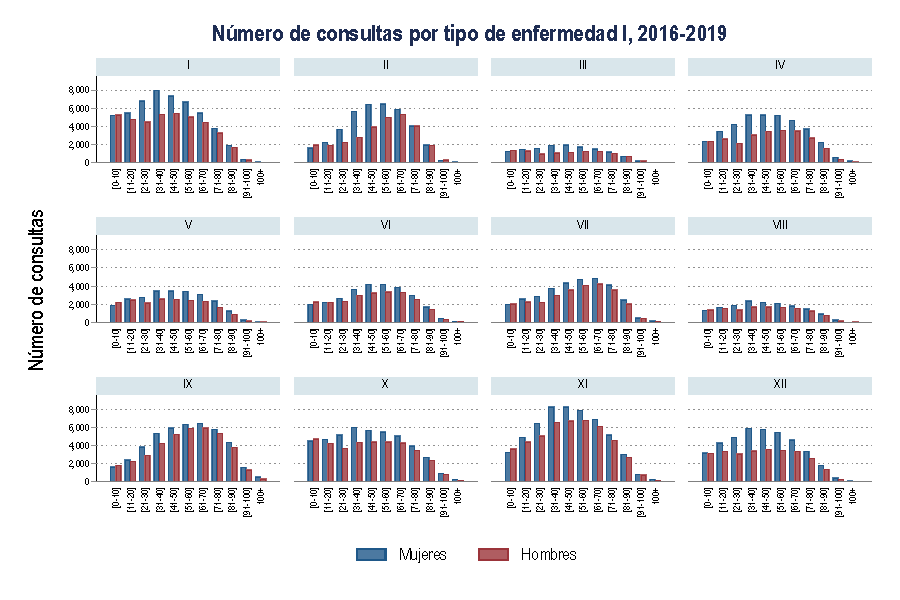
\includegraphics[scale=1.2]{Figures/incidencia_total_1.pdf}
      \begin{tablenotes}
       \item \scriptsize{\textbf{Note:} Number of medical consultations by disease (CIE classification) and sex between 2016-2019. \textbf{Source:} SISALRIL.}  
      \end{tablenotes}
    \end{threeparttable}
\end{figure}


\begin{figure}[H]
    \centering
        \caption{\label{fig: Consultas2} Number of medical consultations by disease and sex II, 2016-2019 }
         \hspace{-2cm}
    \begin{threeparttable}
      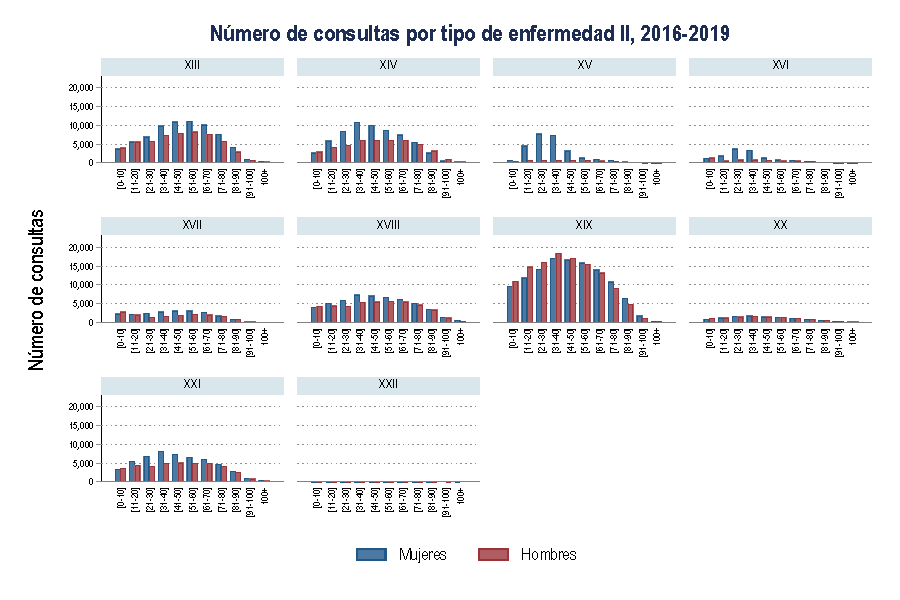
\includegraphics[scale=1.2]{Figures/incidencia_total_2.pdf}
      \begin{tablenotes}
       \item \scriptsize{\textbf{Note:} Number of medical consultations by disease (CIE classification) and sex between 2016-2019. \textbf{Source:} SISALRIL.}  
      \end{tablenotes}
    \end{threeparttable}
\end{figure}

Life expectancies adjusted for the population at risk underlying each disease are found in Table \ref{Tab: LE}. While it is true that life expectancies are similar across categories, it is important to note that all the estimated life expectancies are slightly higher than those of the general population. This detail is significant because, without the adjustment, we would be overestimating the years of life lost. Moreover, there are specific diseases where the correction yields very different results. This is the case, for example, with category IX (Diseases of the circulatory system), where the life expectancy is much higher than normal (exceeding 80 years for both sexes), since it is a type of disease particularly common in older individuals. Finally, it is important to note that all the estimated life expectancies are higher than those reported for the general population. The reason for this is that life expectancies increase once a certain age has been reached (e.g., the life expectancy at birth for a man is $71.07$ years, but once he has reached 50 years old, that expectancy rises to $77.73$), and knowing that a person has a specific disease is informative of their age. \\


\begin{table}[H]
    \caption{\label{Tab: LE} Life expectancy conditional to disease and sex.}
    \centering
    \scalebox{0.8}{
    \setlength{\extrarowheight}{1pt}
    \begin{tabular}{llc}
\toprule[1.5 pt]
\textbf{CIE category} & \textbf{Sex} & \textbf{Life expectancy} \\
\midrule
I                  & F             & 81.11                               \\
                   & M             & 78.00                               \\
II                 & F             & 82.09                               \\
                   & M             & 79.98                               \\
III                & F             & 81.70                               \\
                   & M             & 79.01                               \\
IV                 & F             & 82.20                               \\
                   & M             & 79.23                               \\
V                  & F             & 81.76                               \\
                   & M             & 78.21                               \\
VI                 & F             & 82.27                               \\
                   & M             & 79.17                               \\
VII                & F             & 82.77                               \\
                   & M             & 79.93                               \\
VIII               & F             & 81.86                               \\
                   & M             & 78.81                               \\
IX                 & F             & 83.84                               \\
                   & M             & 81.14                               \\
X                  & F             & 82.06                               \\
                   & M             & 79.01                               \\
XI                 & F             & 82.01                               \\
                   & M             & 79.09                               \\
XII                & F             & 81.55                               \\
                   & M             & 78.49                               \\
XIII               & F             & 82.26                               \\
                   & M             & 79.03                               \\
XIV                & F             & 81.57                               \\
                   & M             & 79.62                               \\
XV                 & F             & 79.46                               \\
                   & M             & 77.54                               \\
XVI                & F             & 79.64                               \\
                   & M             & 77.08                               \\
XVII               & F             & 81.32                               \\
                   & M             & 78.30                               \\
XVIII              & F             & 82.49                               \\
                   & M             & 79.74                               \\
XIX                & F             & 81.78                               \\
                   & M             & 78.01                               \\
XX                 & F             & 81.99                               \\
                   & M             & 78.55                               \\
XXI                & F             & 81.99                               \\
                   & M             & 79.33                               \\
XXII               & F             & 80.34                               \\
                   & M             & 77.28 \\
\bottomrule                   
\end{tabular}
    }
\end{table}

Now, an individual may have multiple diseases reported as the cause of death. In such cases, we take the lowest life expectancy among all those predicted for each disease the individual has. This is because we consider the population with the highest risk as the one that best reflects the individual's health conditions.\\

For the analyses that will be conducted in the rest of the document, it is necessary to move away from the individual as the unit of analysis, and instead consider the impact of diseases on health at a more aggregated level, such as a municipality or province. For this, the measure suggested by \citet{Claxton2015} is to use the sum of all the years of life lost recorded in the desired cell.\footnote{By cell, we refer to a particular level of aggregation. For example, this can be at the municipality-disease-year level, municipality-disease, year, etc.}\\

A first attempt to achieve the total YLL in a given cell would be to consider only premature deaths, that is, those that occur before the estimated life expectancy, since only these represent years of life lost. However, this calculation has a problem, as it does not take into account that many of the deaths observed at a certain age would have occurred, even in the absence of disease, before the estimated life expectancy. It also fails to account for the fact that many of the deaths observed at ages beyond the life expectancy would have occurred without the disease. Therefore, a calculation that better reflects the burden caused by the disease focuses on those deaths that are due to the disease itself, which we can call the excess deaths.\\

\citet{Claxton2015} proposes that a simple way to account for excess deaths is to refer to net YLL, which results from adding both the years lost due to disease when the death is premature and the years of life gained ($\text{YLG}$) when death occurs after the life expectancy ($\text{YLL}_{\text{net}}=\text{YLL}-\text{YLG}$). 
In cases where there are multiple causes of death, we take the one with the highest mortality in the Dominican Republic according to the mortality database of \citet{WHO2022}. The calculations for these indicators in the Dominican Republic are presented in Table \ref{Tab: YLL}.\\

\begin{table}[H]
    \caption{\label{Tab: YLL} Total years of life lost due to excess deaths per disease, 2016-2019}
    \centering
    \hspace*{-0.8cm}
    \scalebox{0.8}{
    \setlength{\extrarowheight}{1pt}
    \begin{threeparttable}
     \hspace{-0.6mm}\begin{tabular}{lllllllll}
\midrule[1.5 pt]
\textbf{Category} & \textbf{Type of} &\textbf{YLL} & \textbf{YLG} & \textbf{Net YLL} & \textbf{YLL} & \textbf{Excess of} & \textbf{Total deaths} & \textbf{Percentage} \\
\textbf{CIE-10} & \textbf{disease} &  &  &  & \textbf{per death} & \textbf{deaths} & & \textbf{excess} \\
 &  &  &  &  & \textbf{observed} &  & &  \\
\midrule
I                      & Infecciosas      & 188,884      & 9,052              & 179,831            & 24.47             & 7,350                   & 8,553  & 85.93       \\
II                     & Cancerígenas     & 252,701      & 17,470             & 235,230            & 18.88             & 12,461                  & 14,956 & 83.32       \\
III                    & Sanguíneas       & 15,451       & 1,006              & 14,444             & 24.82             & 582                     & 677    & 85.97       \\
IV                     & Endocrinas       & 92,695       & 4,505              & 88,190             & 17.24             & 5,115                   & 5,822  & 87.86       \\
V                      & Mentales         & 1,499        & 116                & 1,383              & 23.44             & 59                      & 75     & 78.67       \\
VI                     & Nerviosas        & 19,616       & 1,609              & 18,006             & 22.82             & 789                     & 986    & 80.02       \\
VII                    & Oculares         & 0            & 0                  & 0                  & 0                 & 0                       & 0      & 0.00        \\
VIII                   & Óticas           & 0            & 0                  & 0                  & 0                 & 0                       & 0      & 0.00        \\
IX                     & Circulatorias    & 751,786      & 125,076            & 626,710            & 13.21             & 47,457                  & 65,229 & 72.75       \\
X                      & Respiratorias    & 190,671      & 29,312             & 161,359            & 16.61             & 9,717                   & 13,469 & 72.14       \\
XI                     & Digestivas       & 45,047       & 3,878              & 41,169             & 17.42             & 2,363                   & 2,876  & 82.16       \\
XII                    & Dermatológicas   & 616          & 109                & 507                & 16.37             & 31                      & 36     & 86.11       \\
XIII                   & Osteomusculares  & 2,606        & 258                & 2,348              & 27.63             & 85                      & 112    & 75.89       \\
XIV                    & Genitourinarias  & 62,247       & 3,408              & 58,839             & 22.63             & 2,600                   & 3,016  & 86.21       \\
XV                     & Embarazo y parto & 7,454        & 76                 & 7,377              & 49.52             & 149                     & 151    & 98.68       \\
XVI                    & Perinatales      & 14,060       & 1,532              & 12,527             & 70.38             & 178                     & 223    & 79.82       \\
XVII                   & Malformaciones   & 2,674        & 376                & 2,297              & 45.06             & 51                      & 64     & 79.69       \\
XVIII                  & Otras            & 153,318      & 20,436             & 132,881            & 18.57             & 7,154                   & 9,416  & 75.98       \\
XX                     & Causas externas  & 3,067        & 1,183              & 1,884              & 22.98             & 82                      & 123    & 66.67 \\
\bottomrule
\end{tabular}

     \begin{tablenotes}
     \item \textbf{Note:} $\text{YLL}$, $\text{YLG}$, and $\text{YLL}_{\text{net}}$ per ICD disease category between 2016 and 2019. The table shows average $\text{YLL}$ per death, that is, the average of years of life lost per each premature death. Excess deaths are the number of deaths before expected according to the disease in the mortality table. The average of YLL per premature death is estimated by dividing column 3 by column 5. And the last column is obtained by dividing column 5 by column 6, the percentage of total deaths caused by a disease. 
     \end{tablenotes}
    \end{threeparttable}
    }
\end{table}

\subsubsection{Years of life lost adjusted by quality of life}

Years of life lost (YLL) due to premature death are not a fair measure of the burden a disease imposes on the health system since they weigh each year of life equally. However, not all years are lived with the same quality, so they should not be valued the same. This adjustment is important because it would overestimate the effects of health spending by attributing improvements in health that are not feasible given the person’s age or sex.\\

To address this issue, it is common to transition from YLL to years of life lost adjusted for quality of life (QALYs). To do this, it is necessary to estimate a score associated with the quality of life related to the health states experienced by the general population. This score is a number between 0 and 1, where 1 reflects a state of perfect health, and it decreases with age and varies by sex \parencite{Martin2021}.\\

To obtain these scores, it is common to use forms like EQ-5D, which can calculate an index reflecting the individual's health status. However, such information is not available for the Dominican Republic, so we must necessarily make some kind of approximation.\\

Like \citet{Espinosa2021} and \citet{Martin2021}, we use the quality of life scores presented in \citet{Claxton2015}. Now, since these weights were calculated using a sample from the United Kingdom and are over a decade old, we decided to adjust the weights to better reflect the current reality of the Dominican Republic. For this, we referred to the study by \citet{Bailey2022}, which calculates quality of life weights for 5 Caribbean countries: Barbados, Belize, Colombia, Jamaica, and Trinidad and Tobago. However, the resulting weights are too aggregated to make good adjustments. Consequently, we adjusted the series from \citet{Claxton2015} to reflect the average scores for each age group and sex based on the average scores found in the Caribbean countries. The result of this correction is shown in Figure \ref{fig: pesos}.



\begin{figure}[H]
    \centering
        \caption{\label{fig: pesos} Quality of life score by age and sex.}
    \begin{threeparttable}
      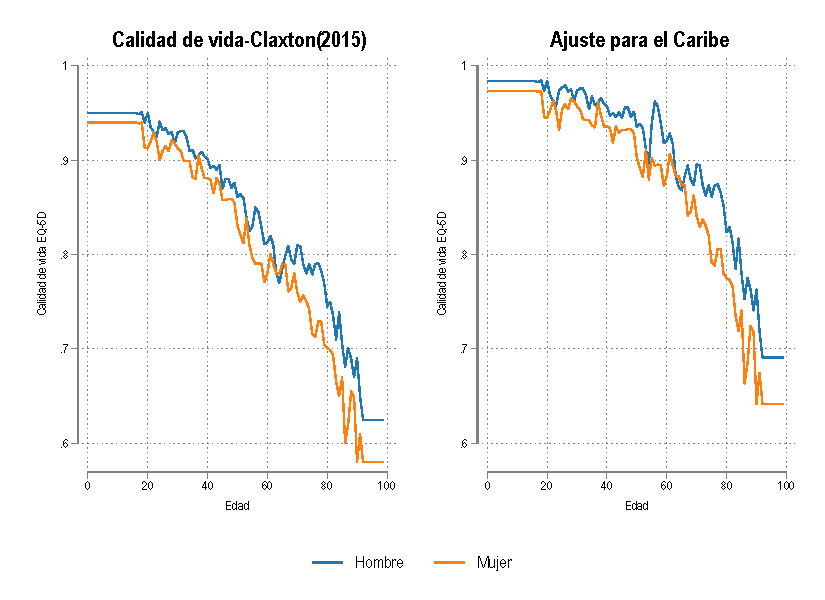
\includegraphics[scale=1.2]{Figures/QOL_graph.pdf}
      \begin{tablenotes}
       \item \scriptsize{\textbf{Note:} Scores in the left panel are those of \citet{Claxton2015}. The right panel shows the adjusted scores so that they reflect the average observed for Caribbean countries from \citet{Bailey2022}.}  
      \end{tablenotes}
    \end{threeparttable}
\end{figure}

More formally, the previous methodologies allow us to calculate the weighting of each year of life by age and sex, which we will denote as $Q_{a,s} \in [0,1]$.\\

Thus, we can calculate the QALYs as:

$$\text{QAYLL}_i=\sum \limits_{a=M_i}^{L_i} Q_{a,S_i}$$

where $L_i=\mathbbm{E}[M_i|S_i=s,E_i]$ is the life expectancy calculated in Table \ref{Tab: LE}. We refer to this quality-adjusted mortality burden as AVAC in what follows.\\

Naturally, introducing quality of life makes the amount of years of life lost smaller compared to when all years are given the same weight. Similarly, the years gained, understood as those occasions when the individual exceeds their life expectancy, will be reduced since those years are not lived in perfect health. As a result, the net years of life lost, adjusted for quality of life, will be less than their unweighted counterparts. A comparison of these measures for the Dominican case is shown in Table \ref{Tab: QALY}.
\begin{table}[H]
    \caption{\label{Tab: QALY} YLL \textit{vs}. YLL adjusted by quality of life, 2016-2019}
    \centering
    \scalebox{0.8}{
    \setlength{\extrarowheight}{1pt}
    \begin{threeparttable}
     
\begin{tabular}{ll @{\hskip 0.5in}lll@{\hskip 0.5in} lll}
\toprule[1.5 pt]
&  & \multicolumn{3}{c}{{\ul\textbf{Sin ajustar}}}   & \multicolumn{3}{c}{{\ul \textbf{Ajustados por calidad de vida}}} \\
\textbf{Categoría} & \textbf{Tipo de} & \textbf{AVP} & \textbf{AVG} & \textbf{AVP netos} & \textbf{AVP}       & \textbf{AVG}      & \textbf{AVP netos}      \\
\textbf{CIE-10}& \textbf{enfermedad} & & &\textbf{} & & & \textbf{}\\
\midrule
I                      & Infecciosas      & 188,884      & 9,052              & 179,831            & 166,353           & 6,953                   & 159,399 \\
II                     & Cancerígenas     & 252,701      & 17,470             & 235,230            & 213,957           & 14,604                  & 199,353 \\
III                    & Sanguíneas       & 15,451       & 1,006              & 14,444             & 13,475            & 778                     & 12,698  \\
IV                     & Endocrinas       & 92,695       & 4,505              & 88,190             & 79,062            & 3,478                   & 75,584  \\
V                      & Mentales         & 1,499        & 116                & 1,383              & 1,324             & 97                      & 1,227   \\
VI                     & Nerviosas        & 19,616       & 1,609              & 18,006             & 17,249            & 1,222                   & 16,027  \\
VII                    & Oculares         & 0            & 0                  & 0                  & 0                 & 0                       & 0       \\
VIII                   & Óticas           & 0            & 0                  & 0                  & 0                 & 0                       & 0       \\
IX                     & Circulatorias    & 751,786      & 125,076            & 626,710            & 633,209           & 97,811                  & 535,398 \\
X                      & Respiratorias    & 190,671      & 29,312             & 161,359            & 165,885           & 22,324                  & 143,561 \\
XI                     & Digestivas       & 45,047       & 3,878              & 41,169             & 39,119            & 2,978                   & 36,141  \\
XII                    & Dermatológicas   & 616          & 109                & 507                & 521               & 77                      & 443     \\
XIII                   & Osteomusculares  & 2,606        & 258                & 2,348              & 2,276             & 192                     & 2,084   \\
XIV                    & Genitourinarias  & 62,247       & 3,408              & 58,839             & 54,205            & 2,707                   & 51,498  \\
XV                     & Embarazo y parto & 7,454        & 76                 & 7,377              & 6,583             & 52                      & 6,532   \\
XVI                    & Perinatales      & 14,060       & 1,532              & 12,527             & 12,812            & 1,046                   & 11,766  \\
XVII                   & Malformaciones   & 2,674        & 376                & 2,297              & 2,442             & 265                     & 2,178   \\
XVIII                  & Otras            & 153,318      & 20,436             & 132,881            & 131,524           & 15,807                  & 115,717 \\
XX                     & Causas externas  & 3,067        & 1,183              & 1,884              & 2,764             & 856                     & 1,908  \\  \bottomrule            
\end{tabular}

     \begin{tablenotes}
     \item \textbf{Note:} Comparison between years of life lost \textit{vs.} years of life lost adjusted for quality of life, by ICD-10 disease category.
     \end{tablenotes}
    \end{threeparttable}
    }
\end{table}

\subsubsection{Disability-Adjusted Life Years}

Now, a disease not only affects an individual by causing premature death but also reduces the quality of life of individuals even while they are still alive. Therefore, an additional adjustment to the measure of disease burden is needed to better reflect the impact of a particular disease. To address this concern, a final adjustment is made to the QALYs measure, known as years lived with disability (YLD). Intuitively, a YLD represents the number of years \emph{in perfect health} that are lost due to a disease. \\

To calculate YLDs, one must add the years of life lost due to premature death to the years lost due to disease $j$ while alive (which we denote as $\text{YLD}_{i,j}$\footnote{A YLD (Years Lived with Disability) represents the years of quality-adjusted life lost by an individual in a year due to the disease, multiplied by the average duration of the disease.}):

\[\text{AVAD}_i=\text{AVAC}_i+\text{YLD}_{i,E_i}\]

To obtain $(\text{YLD}_{i,j})$, we use the estimates for the Dominican Republic available in \citet{GBDC2019}. As \citet{Claxton2015} notes, there are two significant limitations to this source of information. The first is that the codes used to classify diseases are different from those in the ICD-10, so a conversion between the two systems is necessary. Fortunately, the same center provides a table that allows for the conversion between the categories. The second limitation is that these years of life are not measured on the same scale as QALYs, as they do not come from EQ-5D forms, so the authors suggest keeping this in mind when interpreting the results. In the case that an individual suffers from multiple diseases, the years lost for each disease are added together. \\

Beyond being a direct measure of the burden a particular disease imposes on the system, \citet{Claxton2015} indicates that YLDs are useful for understanding \emph{how} the disease causes problems in society. To do this, it is suggested to calculate the ratio given by:

\[R_i=\dfrac{AVAD_i}{AVP_i}=\dfrac{AVAC_i}{AVP_i}+\dfrac{YLD_i}{AVP_i}\]

Note that, by construction, $0<\frac{AVAC}{AVP}<1$, but $\frac{YLD_i}{AVP_i}$ can have arbitrary magnitude. If $R_i=1$, this means that every year lost due to death would have been lived in perfect health. If $R_i<1$, the ratio suggests that most of the burden the disease imposed on the individual was due to premature death. Conversely, if $R_i>1$, this implies that the burden the disease imposed on the individual was mostly due to the loss of quality of life while living with the disease. The distribution of these ratios for the Dominican case is shown for each ICD category in Table~\ref{Tab: Ratios}.
\begin{table}[H]
    \caption{\label{Tab: Ratios} Disease burden ratios by disease type, 2016--2019}
    \centering
    \scalebox{0.8}{
    \setlength{\extrarowheight}{1pt}
    \begin{threeparttable}
     \begin{tabular}{l l c c c}
\toprule[1.5pt]
& &\multicolumn{3}{c}{{\ul \textbf{ Mediana [Percentil 5, Percentil 95]}}} \\
\multicolumn{1}{c}{\textbf{Categoría}} & \textbf{Tipo de} & \textbf{Carga durante vida} & \textbf{Carga por} & \textbf{Carga total} \\ 
\textbf{ CIE-10} &\textbf{enfermedad} &  & \textbf{muerte prematura} & \\ \hline
\\
\ I & Infecciosas & 0.02 [ 0.00, 1.08] &  0.88 [ 0.77, 0.92] &  0.91 [ 0.81, 1.92] \\
\\
\ II &  Cancerígenas & 0.02 [ 0.00, 0.47] &  0.84 [ 0.66, 0.89] &  0.87 [ 0.74, 1.26] \\
\\
\ III & Sanguíneas &  0.01 [ 0.00, 0.85] &  0.87 [ 0.66, 0.92] &  0.89 [ 0.75, 1.74] \\
\\
\ IV & Endocrinas &  0.46 [ 0.13, 3.73] &  0.85 [ 0.71, 0.90] &  1.30 [ 1.01, 4.59] \\
\\
\ V & Mentales &  0.02 [ 0.00, 1.45] &  0.89 [ 0.57, 0.92] &  0.91 [ 0.75, 2.36] \\
\\
\ VI & Nerviosas & 0.06 [ 0.00, 1.00] &  0.87 [ 0.71, 0.92] &  0.93 [ 0.84, 1.77] \\
\\
\ IX & Circulatorias &  0.09 [ 0.00, 2.30] &  0.83 [ 0.50, 0.90] &  0.93 [ 0.77, 3.03] \\
\\
\ X & Respiratorias &  0.04 [ 0.00, 1.83] &  0.87 [ 0.71, 0.92] &  0.91 [ 0.80, 2.63] \\
\\
\ XI & Digestivas &  0.75 [ 0.00, 9.68] &  0.87 [ 0.73, 0.91] &  1.62 [ 0.81,10.52] \\
\\
\ XII & Dematológicas &  0.01 [ 0.00, 0.31] &  0.80 [ 0.00, 0.89] &  0.85 [ 0.50, 0.97] \\
\\
\ XIII & Osteomusculares &  0.03 [ 0.01, 0.48] &  0.87 [ 0.76, 0.91] &  0.91 [ 0.82, 1.35] \\
\\
\ XIV & Genitourinarias &  0.08 [ 0.00, 0.97] &  0.87 [ 0.73, 0.92] &  0.96 [ 0.83, 1.81] \\
\\
\ XV & Embarazo y parto &  0.29 [ 0.00, 1.27] &  0.88 [ 0.87, 0.90] &  1.17 [ 0.89, 2.14] \\
\\
\ XVI & Perinatales &  0.64 [ 0.16, 0.80] &  0.91 [ 0.91, 0.91] &  1.56 [ 1.07, 1.72] \\
\\
\ XVII & Malformaciones &  0.01 [ 0.00, 0.31] &  0.91 [ 0.00, 0.94] &  0.92 [ 0.84, 1.21] \\
\\
\ XVIII & Otras & 0.01 [ 0.00, 0.99] &  0.84 [ 0.62, 0.91] &  0.87 [ 0.70, 1.77] \\
\\
\ XX & Causas externas &  0.01 [ 0.00, 0.03] &  0.91 [ 0.74, 0.93] &  0.91 [ 0.82, 0.95] \\
\\
\midrule[1 pt]
\end{tabular}

    \end{threeparttable}
    }
\end{table}

\subsubsection{Standardized Rate of Healthy Life Years Lost}

Finally, the last step is to aggregate AVAD into a measure that summarizes the impact of a disease in a specific place and year. For this, \citet{Marshall2010} and \citet{Claxton2015} state that two aspects are important: 1) The measure should be interpretable as years of life lost in a particular year (so it makes sense to compare with expenditures in a given year), 2) It should reflect the population structure of the place.

In the previous steps, we described how to calculate the years lived with disability for an individual $i$ who dies at age $a$ due to disease $j$ in municipality $m$ in year $t$, which we denote as $\text{AVAD}_{i}=\text{AVAD}_{i,a,j,m,t}$. Now, we need to calculate the standardized rate of healthy years lost $\text{TAVPE}_{j,m,t}$, incorporating the information available for each individual. We define some quantities of interest:

\begin{itemize}

    \item $\text{AVAD}_{a,j,m,t}$: The total healthy years lost in the population of age $a$, in municipality $m$, due to disease $j$ in year $t$. This is the sum of all net $\text{AVAD}$ lost in that population.
    
    \item $P_{a,j,m,t}$: The number of deaths of people aged $a$, in municipality $m$, due to disease $j$ in year $t$.

    \item $P^*_{a,m}$: The number of people aged $a$ in the population of municipality $m$. This information is available from ONE. Thus, the total number of people in the municipality is

    \[P_m^*= \sum \limits_{a} P^*_{a,m}\]

\end{itemize}

Thus:

\[\text{TAVPE}_{j,m,t}= \sum \limits_{a} \left( \dfrac{\text{AVAD}_{a,j,m,t}}{P_{a,j,m,t}} \right) \left( \dfrac{P^*_{a,m}}{P^*_m} \right)\]

In simple terms, the first term in parentheses represents the years of healthy life lost due to death in an age group, and the second term indicates the weight of that group in the municipality's population. Thus, $\text{TAVPE}_{j,m,t}$ is interpreted as \emph{the number of years of perfect health lost due to a disease, per person in a particular year}.

\subsection{Step 2: Estimating Elasticity}

A key step in calculating the CET is to relate how effective health spending is in reducing the burden of diseases. Traditionally, this relationship is represented by an elasticity, which links how percentage changes in per capita spending translate to percentage changes in the burden a disease imposes on the system. Econometrically, this elasticity can be estimated using a linear regression model given by:

\[\sinh^{-1}(\text{TAVPE}_{j,m,t})=\beta\sinh^{-1}(G_{j,m,t})+ \delta_{j}+\lambda_{m,t}+\epsilon_{j,m,t}\]

where $G_{j,m,t}$ is the spending per patient (in 2016 constant prices) allocated to treat disease $j$ in municipality $m$ in year $t$. $\delta_j$ represents fixed effects of the disease, while $\lambda_{m,t}$ models differential time trends for a municipality (e.g., its population, public spending, etc.).\footnote{For estimation, we use a multiplicative structure for fixed effects, i.e., we take the interaction between municipality and year indicators: $\lambda_{m,t}=\gamma_m\times \zeta_t$.} We opt for this fixed effects structure because it considers many omitted variables reflecting the demand for health services, such as population density, income distribution, municipal budget, among others.

The target parameter is $\beta$, which can be interpreted as the elasticity of health spending after a slight adjustment.\footnote{For elasticity estimation, it is common to use a log-log specification, i.e., estimating a regression with dependent and independent variables transformed by a logarithm. However, this transformation is not possible in this case due to several zeros in the data. Since the arcsinh (inverse hyperbolic sine) allows for including zeros and estimating elasticity with a slight adjustment, this is the preferred approach. This transformation is also used by \citet{Espinosa2021}.} However, estimating this quantity is challenging due to a clear endogeneity problem in the model. For example, higher spending results in better health outcomes, but health disturbances or historical mortality also lead to higher spending. Thus, ordinary least squares estimation of the model would result in inconsistent estimators for the parameter of interest.

To address the endogeneity problem, we use the instrumental variables method. Note that this solution is commonly used in the literature to resolve the endogeneity issue \parencite{Claxton2015,Martin2021,Espinosa2021}. However, we propose different instrumental variables based on a geographical exclusion principle, as in \citet{Benson2019}:

\begin{itemize}
    \item \textbf{Geographic Neighbors:} For each municipality $m \in \mathcal{M}=\{1, \cdots, M\}$, we define $\mathcal{N}(m) \subseteq \mathcal{M}$ as the set of geographic neighbors of $m$. Additionally, we assume that the relationship defined by geographic proximity is not reflexive, i.e., $m \not \in \mathcal{N}(m)$. We define the average spending of the neighbors of $m$, in category $j$ and year $t$ as

\[Z_{m,j,t}= \begin{cases}
\dfrac{1}{\# |\mathcal{N}(m)|} \sum \limits_{n \in \mathcal{N}(m)} G_{n,j,t} & \text{ if } \mathcal{N}(m) \neq \emptyset,\\
0 & \text{ otherwise. }
\end{cases}\]



\begin{figure}[H]
    \centering
        \caption{\label{fig: DistEMuj} Network of geographic neighbors}
    \begin{threeparttable}
      \includegraphics[scale=0.5]{Figures/Network.pdf}
      \begin{tablenotes}
       \item \scriptsize{\textbf{Note:} Network of municipalities sharing a geographic border.}
      \end{tablenotes}
    \end{threeparttable}
\end{figure}

    \item \textbf{k-nearest geographic neighbors:} Let \(N_k(m)\) be the set of the \(k\)-nearest municipalities (excluding \(m\)) according to Euclidean distance. We define the instrument of the \(k\)-nearest neighbors as:

\[Z_{m,j,t}= 
\dfrac{1}{k} \sum \limits_{n \in N_k(m)} G_{n,j,t}\]

    \item \textbf{Inverse distance weighting:} In this case, we consider all municipalities simultaneously but weigh their contribution inversely proportional to the distance between each pair of municipalities. The logic behind this aggregation is to give more importance to the nearest municipalities, as they are the most similar to the municipality of interest. Let \(d(m,m')\) be the distance between municipalities \(m\) and \(m'\). We define the corresponding instrument as:

\[Z_{m,j,t}= 
\dfrac{1}{\# |\mathcal{M}|} \sum \limits_{n \in \mathcal{M}, n \neq m} \dfrac{G_{n,j,t}}{d(m,n)}\]

\end{itemize}

The idea is that each \(Z_{m,j,t}\) is the instrument for \(G_{m,j,t}\). Now, using these instruments will solve the endogeneity problem as long as two conditions are met: relevance and exogeneity.

To guarantee relevance, we need \(\text{Cov}(Z_{m,j,t},G_{m,j,t},|\delta_j,\lambda_{m,t}) \neq 0\), meaning that the expenditure observed in a municipality is somewhat correlated with the expenditures observed in neighboring municipalities. This is reasonable since budget increases or cuts generally occur at the national level, as well as government initiatives aimed at addressing a particular disease \(j\).

To satisfy exogeneity, it must be true that \(\text{Cov}(Z_{m,j,t},\epsilon_{m,j,t},|\delta_j,\lambda_{m,t}) = 0\). Briefly, this assumption implies that, given the characteristics of a disease \(j\) (e.g., being very lethal, contagious, etc.) and the natural evolution of a municipality \(m\) over time (e.g., its population, municipal budget, etc.), the expenditure made by neighboring municipalities does not affect the health outcomes observed within the municipality. Since the municipality is not part of its neighbors, \(Z_{m,j,t}\) does not contain the health expenditure used for healthcare services in that municipality. Therefore, it is unlikely that health investments made \emph{in other municipalities} would improve the services provided in the municipality of interest. This is even less likely given the flexibility of fixed effects, where we are looking at reallocations of health spending to a particular disease, given a certain level and trend of overall expenditure.

Finally, since we have different plausible estimators of the parameter \(\beta\) (one for each instrument), we can combine them to increase the precision of our estimate. Specifically, we will use the methodology developed by \citet{Lavancier2016} to produce the most precise estimate possible of the cost-effectiveness threshold. A brief explanation of the method is included in Appendix \ref{S: Comb}.

\subsection{Step 3: Calculation of the cost-effectiveness threshold}

As a final step, we will use the results of the previous model to estimate the cost-effectiveness threshold, as suggested by \citet{Claxton2015}. The cost-effectiveness threshold is given by

\[k=\dfrac{\Delta G}{\Delta \text{TAVPE}}=\dfrac{\bar{G}}{\hat{\xi} \;\overline{\text{TAVPE}}}=\dfrac{\sqrt{1+\bar{G}^2}}{\hat{\beta} \; \sqrt{1+\overline{\text{TAVPE}}^2}  }\]

where \(k\) represents the health expenditure necessary to reduce one unit of \(\text{TAVPE}\). This equals the ratio of average health expenditure \((G)\) to the average change in the health burden per unit change in expenditure \((\hat{\xi}\; \overline{\text{TAVPE}})\), where \(\hat{\xi}\) is the estimated expenditure elasticity of TAVPE. The \(\hat{\beta}\) is the parameter of the model estimated using two-stage least squares. The detailed proof of this formula is found in Appendix \ref{S: Cálculo}.

\section{Results}

Based on the strategy described in Section 3, we proceed to estimate the CET for the Dominican Republic. The main results are reported in Table~\ref{Tab: TabIV}.\footnote{All specifications in Table~\ref{Tab: TabIV} use $N = 10{,}626$ observations. The four missing observations relative to specifications with separate municipality and year fixed effects ($N = 10{,}630$) correspond to disease-municipality-year cells with a single observation (singletons), which are automatically absorbed and excluded when both fixed effects are interacted.} Each column corresponds to implementing the methodology described in Section~3.2 under a different choice of instrument. Panel~A reports the estimate of parameter $\beta$ obtained from the two-stage least squares procedure, while Panel~B reports the expenditure elasticity derived following the adjustment described in Appendix~\ref{S: Cálculo}. Panel~C reports the estimated CET together with its standard error and 95\% confidence interval. The instrument is sufficiently relevant across all specifications, as the Kleibergen-Paap $F$-statistic exceeds the threshold of $16.38$ recommended by \citet{StockYogo2005}. Regressions are weighted by each municipality's total population.\footnote{\citet[p.200]{Claxton2015} emphasize the importance of rescaling the regression to account for the different population sizes that each municipality represents within the health system.}\\

The point estimates of the threshold derived from the different instruments are relatively similar. Moreover, the fact that all confidence intervals overlap indicates that the estimation is not sensitive to the choice of instrument, as the estimates are statistically indistinguishable from one another. The point estimates across the four IV strategies range from 86,498 to 107,824 Dominican pesos, equivalent to between 26\% and 33\% of per capita GDP in 2016 (330,949 Dominican pesos).\footnote{Banco Central de la República Dominicana (BCRD), Cuentas Nacionales. Available at \href{https://www.bancentral.gov.do/a/d/2533-sector-real}{https://www.bancentral.gov.do/a/d/2533-sector-real}.}\footnote{At the 2016 annual average exchange rate of approximately 46.5 DOP per USD (BCRD), the preferred estimate of 86,498 DOP is equivalent to approximately USD~1,860.} Furthermore, the estimate changes little when AVAC is used as an alternative health measure instead of AVAD, as shown in Table~\ref{Tab: TabIV_V2}, in which case the estimated threshold ranges between 108,349 and 138,180 Dominican pesos (between 33\% and 42\% of per capita GDP).



\begin{table}[H]
    \caption{\label{Tab: TabIV} Cost-effectiveness threshold, alternative IV strategies}
    \centering
    \scalebox{0.8}{
    \setlength{\extrarowheight}{1pt}
    \begin{threeparttable}
     \begin{tabular}{l c c c c}
\toprule[1.5pt]
\multicolumn{1}{c}{\textbf{}} & \textbf{(1)} & \textbf{(2)} & \textbf{(3)} & \textbf{(4)}   \\
\multicolumn{1}{c}{\textbf{}} & \textbf{Contiguous} & \textbf{Five nearest} & \textbf{Ten nearest} & \textbf{Inverse-distance}   \\
\multicolumn{1}{c}{\textbf{}} & \textbf{municipalities} & \textbf{neighbors} & \textbf{neighbors} & \textbf{weighting}   \\ \hline \\
\\
\multicolumn{5}{l}{Panel A. \textit{Model parameter}}\\
\\
Model parameter & -0.351 & -0.320 & -0.317 & -0.282  \\
& (0.113) & (0.120)  & (0.131) & (0.117)  \\
\\
\multicolumn{5}{l}{Panel B. \textit{Expenditure elasticity}}\\
\\
Elasticity & -0.356 & -0.324 & -0.321 & -0.285  \\
& (0.114) & (0.122)  & (0.133) & (0.118)  \\
\\
\multicolumn{5}{l}{Panel C. \textit{Cost-effectiveness threshold}}\\
\\
Threshold [Thousands DOP] & 86.498 & 95.022  & 95.870 & 107.824  \\
& (27.763) & (35.822) & (39.621) & (44.659)  \\
& [40.832,132.165] & [36.100,153.944]  & [30.699,161.042]  & [34.366,181.282]   \\
\\
\midrule[1 pt]
\\
Observations & 10626 & 10626 &  10626 & 10626 \\
Kleibergen-Paap F & 155.95 & 54.67 & 18.73 & 26.98 \\
\\
\midrule[1 pt]
\\
\multicolumn{5}{l}{\textit{Fixed effects}} \\
\\
Disease type & $\checkmark$ & $\checkmark$ & $\checkmark$  & $\checkmark$ \\
Municipality $\times$ Year & $\checkmark$   &  $\checkmark$ & $\checkmark$ & $\checkmark$ \\
\\
\midrule[1 pt]
\end{tabular}

     \begin{tablenotes}
     \item \textbf{Note:} Standard errors in parentheses; 95\% confidence intervals in square brackets. In Panel~A, errors are clustered at the municipality level. Standard errors in Panels~B and C are computed using the delta method applied to the Panel~A errors. Regressions are weighted by municipal population in each year. Column~1 is the preferred specification. Column~1 uses contiguous municipalities as the instrument. Columns~2 and 3 use the average per capita expenditure of the 5 and 10 nearest neighbors (by geographic distance), respectively. Column~4 uses average per capita expenditure weighted by the inverse of the distance between each pair of municipalities.
     \end{tablenotes}
    \end{threeparttable}
    }
\end{table}



\begin{table}[H]
    \caption{\label{Tab: TabIV_V2} Cost-effectiveness threshold, alternative IV strategies, AVAC 2016--2019}
    \centering
    \scalebox{0.8}{
    \setlength{\extrarowheight}{1pt}
    \begin{threeparttable}
     \begin{tabular}{l c c c c}
\toprule[1.5pt]
\multicolumn{1}{c}{\textbf{}} & \textbf{(1)} & \textbf{(2)} & \textbf{(3)} & \textbf{(4)}   \\
\multicolumn{1}{c}{\textbf{}} & \textbf{Contiguous} & \textbf{Five nearest} & \textbf{Ten nearest} & \textbf{Inverse-distance}   \\
\multicolumn{1}{c}{\textbf{}} & \textbf{municipalities} & \textbf{neighbors} & \textbf{neighbors} & \textbf{weighting}   \\ \hline \\
\\
\multicolumn{5}{l}{Panel A. \textit{Model parameter}}\\
\\
Model parameter & -0.313 & -0.283 & -0.282 & -0.246  \\
& (0.111) & (0.119)  & (0.127) & (0.112)  \\
\\
\multicolumn{5}{l}{Panel B. \textit{Expenditure elasticity}}\\
\\
Elasticity & -0.318 & -0.288 & -0.286 & -0.250  \\
& (0.112) & (0.121)  & (0.129) & (0.114)  \\
\\
\multicolumn{5}{l}{Panel C. \textit{Cost-effectiveness threshold}}\\
\\
Threshold [Thousands DOP] & 108.349 & 119.959  & 120.614 & 138.180  \\
& (38.235) & (50.452) & (54.477) & (63.170)  \\
& [45.458,171.239] & [36.973,202.946]  & [31.008,210.220]  & [34.275,242.085]   \\
\\
\midrule[1 pt]
\\
Observations & 10626 & 10626 &  10626 & 10626 \\
Kleibergen-Paap F & 155.95 & 54.67 & 18.73 & 26.98 \\
\\
\midrule[1 pt]
\\
\multicolumn{5}{l}{\textit{Fixed effects}} \\
\\
Disease type & $\checkmark$ & $\checkmark$ & $\checkmark$  & $\checkmark$ \\
Municipality $\times$ Year & $\checkmark$   &  $\checkmark$ & $\checkmark$ & $\checkmark$ \\
\\
\midrule[1 pt]
\end{tabular}

     \begin{tablenotes}
     \item \textbf{Note:} Standard errors in parentheses; 95\% confidence intervals in square brackets. In Panel~A, errors are clustered at the municipality level. Standard errors in Panels~B and C are computed using the delta method applied to the Panel~A errors. Regressions are weighted by municipal population in each year. Column~1 is the preferred specification. Column~1 uses contiguous municipalities as the instrument. Columns~2 and 3 use the average per capita expenditure of the 5 and 10 nearest neighbors (by geographic distance), respectively. Column~4 uses average per capita expenditure weighted by the inverse of the distance between each pair of municipalities.
     \end{tablenotes}
    \end{threeparttable}
    }
\end{table}


As a final step, we apply the methodology described in Appendix~\ref{S: Comb}. The results of this exercise are reported in Table~\ref{Tab: Oracle}. The combined estimator for the AVAD measure yields a threshold estimate of 94,615 Dominican pesos, equivalent to 29\% of the country's per capita GDP in 2016. The same exercise using AVAC as an alternative health measure yields a combined threshold estimate of 128,164 Dominican pesos, corresponding to 39\% of per capita GDP.

The weighting pattern in the combined estimator warrants brief comment. Although the contiguous-municipalities instrument achieves the highest first-stage $F$-statistic ($F = 155.95$), it receives a weight of only 12\% in the MSE-minimizing combination, while the 5-nearest-neighbors instrument receives 76\%. This reflects the role of the full variance-covariance matrix $\hat{\Sigma}$ in determining the optimal weights. For most municipalities in the Dominican Republic, the set of contiguous neighbors is a strict subset of the five nearest neighbors, implying that the two instruments share a large fraction of their identifying variation. In a minimum mean-squared-error combination, two highly correlated estimators offer limited diversification benefit relative to a pair with lower correlation; the MSE-minimizing weights therefore concentrate on the 5-nearest-neighbors specification, which captures variation in neighboring expenditure that the contiguous instrument does not.


\begin{table}[H]
    \caption{\label{Tab: Oracle} Cost-effectiveness threshold, combining IV estimators}
    \centering
    \scalebox{0.8}{
    \setlength{\extrarowheight}{1pt}
    \begin{threeparttable}
     \begin{tabular}{l c c}
\toprule[1.5pt]
\multicolumn{1}{c}{\textbf{}} & \textbf{(1)} & \textbf{(2)}  \\
\multicolumn{1}{c}{\textbf{}} &  \textbf{Standardized AVAD} & \textbf{Standardized AVAC}  \\ \hline \\
\\
\multicolumn{3}{l}{Panel A. \textit{Combined cost-effectiveness threshold}}\\
\\
Threshold [Thousands DOP] & 94.615  & 128.164  \\
& (21.41) & (18.415) \\
& [52.640,136.589]  & [92.070,164.257]    \\
\\
Percentage of per capita GDP (2016) &  0.29 &   0.39 \\
\\
\multicolumn{3}{l}{Panel B. \textit{Assigned weights}} \\
\\
Contiguous municipalities &  0.12  &  0.25 \\
Five nearest neighbors &  0.76 &  0.03 \\
Ten nearest neighbors &  0.08 &  0.12 \\
Inverse-distance weighting &  0.04 &  0.60 \\
\\
\bottomrule[1 pt]
\end{tabular}

     \begin{tablenotes}
     \item \textbf{Note:} Combined estimator following the procedure of \citet{Lavancier2016}. The variance-covariance matrix of the estimators is estimated using bootstrap (10,000 replications) with cluster resampling at the municipality level. Standard errors in parentheses; 95\% confidence intervals in square brackets. Column~(1) reports the combined threshold using standardized disability-adjusted life years as the health measure (AVAD). Column~(2) reports the combined threshold using standardized quality-adjusted life years as the health measure (AVAC).
     \end{tablenotes}
    \end{threeparttable}
    }
\end{table}


To further assess the credibility of the results, we conduct several robustness exercises. First, we compare the two-stage least squares estimates with those obtained by ordinary least squares (OLS). The results are reported in Table~\ref{Tab: TabOLS}. As is standard, OLS tends to underestimate the expenditure elasticity in absolute value: the OLS parameter estimate is $-0.003$ (SE $= 0.010$), statistically indistinguishable from zero, compared to the IV estimate of $-0.351$ (Panel~A model parameter) in the preferred specification. Intuitively, this occurs because periods of high fiscal spending are positively correlated with omitted variables reflecting elevated demand for health services: the periods in which the most is spent are precisely those in which the worst health outcomes are observed. As a result, OLS would incorrectly suggest that expenditure is relatively ineffective at reducing the disease burden. This discrepancy justifies the use of instrumental variables---which also confirms their validity, since the bias is corrected in the expected direction---since failing to do so would lead to overestimating the threshold.\\

We also examine the relevance of the instruments in Table~\ref{Tab: First}. The first-stage estimates have the expected sign: fiscal increases in neighboring municipalities are associated with fiscal increases in the municipality of interest. This correlation is statistically significant and strong, as evidenced by the high $t$-statistics. We additionally estimate the reduced form of the model. As argued by \citet{Chernozhukov2008}, the reduced form allows examination of the relationship between expenditure and the disease burden even when the instrument is weak. Consistent with theory, the reduced form indicates a negative relationship between these two variables, confirming that expenditure is effective in reducing the health burden.\\


Finally, we evaluate the exogeneity of the instruments using the $C$-statistic developed by \citet{K.Newey1985} and \citet{Eichenbaum1988}.\footnote{A detailed explanation of the method is provided in \citet{Hayashi2000}, pp.~218--221 and 232--234.} The test requires an auxiliary instrument that satisfies the exogeneity assumption and can therefore be used to evaluate the validity of the remaining instruments. Since the primary threat to identification arises from intermunicipal migration flows, we use the three most distant municipalities as the auxiliary instrument. Although this instrument is considerably weaker than those employed in the main specifications, it is less likely to be contaminated by intermunicipal population flows.\\

Using all instruments simultaneously, as in column~5 of Table~\ref{Tab: Sargan} in the appendix, we can perform a test whose null hypothesis is that all instruments are valid (i.e., all instruments used in the estimation of the threshold), taking the auxiliary instrument as exogenous. Note that adding the weaker auxiliary instrument causes the combined Kleibergen-Paap $F$-statistic to fall below the 16.38 threshold in columns~3 and~4 of Table~\ref{Tab: Sargan} ($F = 9.80$ and $F = 13.79$, respectively), because the ten-nearest-neighbor and inverse-distance instruments are weaker in conjunction with the auxiliary. The validity inference is drawn from column~5, which retains high instrument relevance ($F = 71.03$). We obtain a $C$-statistic of $3.72$ ($p$-value $= 0.44$), which does not allow rejection of the null hypothesis at standard significance levels. This provides evidence that the instruments are valid.\footnote{Validity here refers to the condition that the instruments are uncorrelated with the idiosyncratic error conditional on the fixed effects.} Furthermore, the estimated threshold changes little when the proposed instruments are combined with the auxiliary instrument (see columns~1--4), suggesting that their inclusion does not introduce biases arising from potential correlation with the error term. 

\section{Conclusion}

This study provides the first within-country supply-side estimate of the cost-effectiveness threshold for the Dominican Republic's public health system, and the first such estimate for the Caribbean region. Using data on disease burden, per capita health expenditure, and population structure across municipalities and ICD-10 disease categories for the period 2016--2019, the preferred specification yields a CET of 86,498 Dominican pesos (DOP), equivalent to approximately 26\% of per capita GDP in 2016, with a 95\% confidence interval of 40,832--132,165 DOP (12.3\%--39.9\% of per capita GDP). The combined estimator that pools information across four IV strategies yields a point estimate of 94,615 DOP (29\% of per capita GDP) for the AVAD-based health outcome. Results are robust to alternative health measures (AVAC), alternative IV strategies, and instrument exogeneity tests.

These estimates have direct implications for coverage and pricing decisions under the Plan Básico de Salud. The central estimate of 86,498 DOP lies substantially below the World Health Organization's heuristic of one to three times per capita GDP (approximately 331,000--993,000 DOP at 2016 prices). This gap suggests that the WHO heuristic significantly overstates the marginal cost of producing health within the Dominican system, and that applying it as a coverage threshold would approve technologies whose incremental costs exceed the health benefits they displace. The present estimate is consistent with the cross-country projections of \citet{Woods2016} and \citet{PichonRiviere2023}, both of which predict thresholds below one times per capita GDP for upper-middle-income countries. Compared to Colombia's first within-country supply-side estimate---approximately USD~4,488 per YLL avoided \parencite{Espinosa2021}---the Dominican estimate (approximately USD~1,860 per YLL avoided at 2016 exchange rates) is lower, consistent with the Dominican Republic's position at a lower income level within the upper-middle-income group.

The identification strategy relies on three key assumptions. First, the geographic exclusion restriction requires that neighboring municipalities' disease-specific expenditure affects health outcomes in the focal municipality only through its effect on that municipality's own spending. This assumption is most credible for non-communicable disease categories where cross-municipal disease transmission is minimal; it deserves further scrutiny for infectious and respiratory diseases. Second, the municipality-by-year and disease fixed effects are assumed to absorb all confounders varying along those dimensions; time-varying disease-specific shocks within a municipality that are correlated with neighbor spending remain a potential concern. Third, the quality-of-life weights used to construct AVAC are adapted from Caribbean country averages rather than measured directly in the Dominican Republic, introducing uncertainty into the AVAC-based results reported in Table~\ref{Tab: TabIV_V2}.

The conditions for institutional adoption of this estimate remain to be established. The experience of the nine countries reviewed by \citet{Espinosa2024} suggests that an empirically grounded threshold is a necessary but not sufficient condition for evidence-based HTA: regulatory frameworks, institutional mandates, and stakeholder engagement processes must be developed alongside the empirical work. The present study provides the health authorities of the Dominican Republic with a first domestically grounded reference value that can inform those processes.

Future work can extend this study along several dimensions. A longer panel incorporating data beyond 2019 would allow estimation of lagged expenditure effects, reducing reliance on contemporaneous cross-sectional variation. Following \citet{Espinosa2021}, administrative instruments derived from central regulatory decisions---price ceilings on specific medications or coverage expansions under the Plan Básico de Salud---would provide an additional IV strategy that does not depend on geographic spillover assumptions. Incorporating longitudinal health-related quality-of-life data collected directly in the Dominican Republic would reduce dependence on adapted quality weights and yield a more precise AVAC-based threshold estimate.

\newpage

\printbibliography[title={References}]

\newpage
\appendix
\counterwithin{figure}{section}
\counterwithin{table}{section}

\section{Appendix}

\subsection{Tables and Additional Figures}


\begin{table}[H]
    \caption{\label{Tab: SummaryMortalidad} Descriptive statistics of mortality data}
    \centering
    \scalebox{0.8}{
    \setlength{\extrarowheight}{1pt}
    \begin{threeparttable}
     \begin{tabular}{l c c c c c}
\toprule[1.5pt]
\multicolumn{1}{c}{\textbf{Variable}} & \textbf{Media} & \parbox[c][1.3cm]{3cm}{\centering \textbf{\\ Desviación \\ Estándar \\ }} & \textbf{Mínimo}
&  \textbf{Mediana} & \textbf{Máximo} \\ \hline \\
\\
\multicolumn{6}{l}{Panel A. \textit{Variables principales}}\\
\\
\ Edad Muerte & 57.800 & 28.295 &     0 &    65 &   119 \\
\ Mujer[1=Sí] & 0.410 & 0.492 &     0 &     0 &     1 \\
\ Año de nacimiento & 1959.311 & 28.374 &  1899 &  1952 &  2019 \\
\ Año de muerte & 2017.569 & 1.121 &  2016 &  2018 &  2019 \\
\\
\multicolumn{6}{l}{Panel B. \textit{Tipo muerte}}\\
\\
\ No violenta & 0.846 & 0.361 &     0 &     1 &     1 \\
\ Homicidio & 0.034 & 0.181 &     0 &     0 &     1 \\
\ Suicidio & 0.014 & 0.118 &     0 &     0 &     1 \\
\ Accidente de trabajo & 0.003 & 0.050 &     0 &     0 &     1 \\
\ Accidente de tránsito  & 0.061 & 0.239 &     0 &     0 &     1 \\
\ Otro tipo de accidente  & 0.020 & 0.140 &     0 &     0 &     1 \\
\ Indeterminado  & 0.014 & 0.118 &     0 &     0 &     1 \\
\\
\multicolumn{6}{l}{Panel C. \textit{Número de causas de muertes registradas con códigos CIE por persona fallecida}} \\
\\
\ 0 causas & 0.029 & 0.167 &     0 &     0 &     1 \\
\ 1 causa & 0.209 & 0.406 &     0 &     0 &     1 \\
\ 2 causas & 0.275 & 0.447 &     0 &     0 &     1 \\
\ 3 causas & 0.256 & 0.436 &     0 &     0 &     1 \\
\ 4 causas & 0.161 & 0.367 &     0 &     0 &     1 \\
\ 5 causas & 0.050 & 0.219 &     0 &     0 &     1 \\
\ 6 causas & 0.020 & 0.140 &     0 &     0 &     1 \\
\\
\midrule[1 pt]
\end{tabular}

     \begin{tablenotes}
     \item \textbf{Note:} Number of observations: 179,852.
     \end{tablenotes}
    \end{threeparttable}
    }
\end{table}



\begin{table}[H]
    \caption{\label{Tab: TNV1} National life table I, 2015-2020}
    \centering
    \hspace*{-1cm}
    \scalebox{0.7}{
    \setlength{\extrarowheight}{0.5pt}
    \begin{threeparttable}
     \begin{tabular}{cccc|ccc}
\toprule[1.5 pt]
     & \multicolumn{3}{c}{Men}                                                                                                                                                                                                                                                                       & \multicolumn{3}{c}{Women}                                                                                                                                                                                                                                                                       \\ \hline
Age & \begin{tabular}[c]{@{}c@{}}Probability of\\ death\end{tabular} & \multicolumn{1}{c}{\begin{tabular}[c]{@{}c@{}}Number of people\\ alive (per 100k)\end{tabular}} & \begin{tabular}[c]{@{}c@{}}Expectativa de vida adicional\\ condicional en haber cumplido\\ los años indicados\end{tabular} & \begin{tabular}[c]{@{}c@{}}Probabilidad de\\ muerte\end{tabular} & \multicolumn{1}{c}{\begin{tabular}[c]{@{}c@{}}Número de personas\\ vivas (por 100k)\end{tabular}} & \begin{tabular}[c]{@{}c@{}}Expected additional life\\ conditional to having reached\\  the indicated age\end{tabular} \\
\midrule
0    & 0.02450                                                          & 100,000                                                                                           & 71.07                                                                                                                      & 0.01845                                                          & 100,000                                                                                           & 76.17                                                                                                                      \\
1    & 0.00199                                                          & 97,550                                                                                            & 71.86                                                                                                                      & 0.00170                                                          & 98,183                                                                                            & 76.58                                                                                                                      \\
2    & 0.00135                                                          & 97,356                                                                                            & 71.00                                                                                                                      & 0.00109                                                          & 98,016                                                                                            & 75.71                                                                                                                      \\
3    & 0.00114                                                          & 97,225                                                                                            & 70.09                                                                                                                      & 0.00072                                                          & 97,909                                                                                            & 74.79                                                                                                                      \\
4    & 0.00049                                                          & 97,114                                                                                            & 69.17                                                                                                                      & 0.00044                                                          & 97,838                                                                                            & 73.84                                                                                                                      \\
5    & 0.00035                                                          & 97,066                                                                                            & 68.21                                                                                                                      & 0.00032                                                          & 97,795                                                                                            & 72.87                                                                                                                      \\
6    & 0.00032                                                          & 97,032                                                                                            & 67.23                                                                                                                      & 0.00028                                                          & 97,764                                                                                            & 71.90                                                                                                                      \\
7    & 0.00029                                                          & 97,002                                                                                            & 66.25                                                                                                                      & 0.00025                                                          & 97,737                                                                                            & 70.92                                                                                                                      \\
8    & 0.00028                                                          & 96,973                                                                                            & 65.27                                                                                                                      & 0.00023                                                          & 97,712                                                                                            & 69.93                                                                                                                      \\
9    & 0.00027                                                          & 96,946                                                                                            & 64.29                                                                                                                      & 0.00023                                                          & 97,690                                                                                            & 68.95                                                                                                                      \\
10   & 0.00027                                                          & 96,921                                                                                            & 63.31                                                                                                                      & 0.00023                                                          & 97,667                                                                                            & 67.97                                                                                                                      \\
11   & 0.00030                                                          & 96,894                                                                                            & 62.32                                                                                                                      & 0.00024                                                          & 97,645                                                                                            & 66.98                                                                                                                      \\
12   & 0.00037                                                          & 96,865                                                                                            & 61.34                                                                                                                      & 0.00026                                                          & 97,622                                                                                            & 66.00                                                                                                                      \\
13   & 0.00050                                                          & 96,829                                                                                            & 60.36                                                                                                                      & 0.00029                                                          & 97,596                                                                                            & 65.01                                                                                                                      \\
14   & 0.00066                                                          & 96,781                                                                                            & 59.39                                                                                                                      & 0.00034                                                          & 97,567                                                                                            & 64.03                                                                                                                      \\
15   & 0.00084                                                          & 96,717                                                                                            & 58.43                                                                                                                      & 0.00038                                                          & 97,535                                                                                            & 63.05                                                                                                                      \\
16   & 0.00102                                                          & 96,636                                                                                            & 57.48                                                                                                                      & 0.00043                                                          & 97,498                                                                                            & 62.08                                                                                                                      \\
17   & 0.00122                                                          & 96,538                                                                                            & 56.54                                                                                                                      & 0.00049                                                          & 97,456                                                                                            & 61.10                                                                                                                      \\
18   & 0.00144                                                          & 96,420                                                                                            & 55.61                                                                                                                      & 0.00056                                                          & 97,408                                                                                            & 60.13                                                                                                                      \\
19   & 0.00168                                                          & 96,280                                                                                            & 54.69                                                                                                                      & 0.00064                                                          & 97,353                                                                                            & 59.17                                                                                                                      \\
20   & 0.00192                                                          & 96,119                                                                                            & 53.78                                                                                                                      & 0.00072                                                          & 97,291                                                                                            & 58.21                                                                                                                      \\
21   & 0.00215                                                          & 95,935                                                                                            & 52.88                                                                                                                      & 0.00080                                                          & 97,221                                                                                            & 57.25                                                                                                                      \\
22   & 0.00233                                                          & 95,728                                                                                            & 51.99                                                                                                                      & 0.00088                                                          & 97,144                                                                                            & 56.29                                                                                                                      \\
23   & 0.00244                                                          & 95,505                                                                                            & 51.11                                                                                                                      & 0.00095                                                          & 97,059                                                                                            & 55.34                                                                                                                      \\
24   & 0.00249                                                          & 95,272                                                                                            & 50.24                                                                                                                      & 0.00101                                                          & 96,967                                                                                            & 54.39                                                                                                                      \\
25   & 0.00253                                                          & 95,034                                                                                            & 49.36                                                                                                                      & 0.00108                                                          & 96,869                                                                                            & 53.45                                                                                                                      \\
26   & 0.00257                                                          & 94,794                                                                                            & 48.49                                                                                                                      & 0.00115                                                          & 96,764                                                                                            & 52.50                                                                                                                      \\
27   & 0.00261                                                          & 94,550                                                                                            & 47.61                                                                                                                      & 0.00121                                                          & 96,653                                                                                            & 51.56                                                                                                                      \\
28   & 0.00266                                                          & 94,303                                                                                            & 46.73                                                                                                                      & 0.00128                                                          & 96,536                                                                                            & 50.63                                                                                                                      \\
29   & 0.00271                                                          & 94,052                                                                                            & 45.86                                                                                                                      & 0.00134                                                          & 96,413                                                                                            & 49.69                                                                                                                      \\
30   & 0.00276                                                          & 93,797                                                                                            & 44.98                                                                                                                      & 0.00140                                                          & 96,284                                                                                            & 48.76                                                                                                                      \\
31   & 0.00281                                                          & 93,538                                                                                            & 44.10                                                                                                                      & 0.00147                                                          & 96,149                                                                                            & 47.82                                                                                                                      \\
32   & 0.00286                                                          & 93,276                                                                                            & 43.23                                                                                                                      & 0.00154                                                          & 96,008                                                                                            & 46.89                                                                                                                      \\
33   & 0.00293                                                          & 93,009                                                                                            & 42.35                                                                                                                      & 0.00161                                                          & 95,861                                                                                            & 45.97                                                                                                                      \\
34   & 0.00302                                                          & 92,736                                                                                            & 41.47                                                                                                                      & 0.00168                                                          & 95,707                                                                                            & 45.04                                                                                                                      \\
35   & 0.00311                                                          & 92,456                                                                                            & 40.60                                                                                                                      & 0.00176                                                          & 95,546                                                                                            & 44.11                                                                                                                      \\
36   & 0.00321                                                          & 92,168                                                                                            & 39.72                                                                                                                      & 0.00185                                                          & 95,377                                                                                            & 43.19                                                                                                                      \\
37   & 0.00332                                                          & 91,872                                                                                            & 38.85                                                                                                                      & 0.00195                                                          & 95,201                                                                                            & 42.27                                                                                                                      \\
38   & 0.00343                                                          & 91,567                                                                                            & 37.97                                                                                                                      & 0.00206                                                          & 95,016                                                                                            & 41.35                                                                                                                      \\
39   & 0.00355                                                          & 91,253                                                                                            & 37.10                                                                                                                      & 0.00218                                                          & 94,820                                                                                            & 40.43                                                                                                                      \\
40   & 0.00369                                                          & 90,929                                                                                            & 36.23                                                                                                                      & 0.00232                                                          & 94,614                                                                                            & 39.52                                                                                                                      \\
41   & 0.00385                                                          & 90,594                                                                                            & 35.37                                                                                                                      & 0.00248                                                          & 94,394                                                                                            & 38.61                                                                                                                      \\
42   & 0.00403                                                          & 90,245                                                                                            & 34.50                                                                                                                      & 0.00263                                                          & 94,160                                                                                            & 37.71                                                                                                                      \\
43   & 0.00422                                                          & 89,882                                                                                            & 33.64                                                                                                                      & 0.00277                                                          & 93,913                                                                                            & 36.81                                                                                                                      \\
44   & 0.00444                                                          & 89,503                                                                                            & 32.78                                                                                                                      & 0.00290                                                          & 93,654                                                                                            & 35.91                                                                                                                      \\
45   & 0.00467                                                          & 89,106                                                                                            & 31.92                                                                                                                      & 0.00305                                                          & 93,382                                                                                            & 35.01                                                                                                                      \\
46   & 0.00495                                                          & 88,689                                                                                            & 31.07                                                                                                                      & 0.00323                                                          & 93,098                                                                                            & 34.11                                                                                                                      \\
47   & 0.00531                                                          & 88,250                                                                                            & 30.22                                                                                                                      & 0.00349                                                          & 92,797                                                                                            & 33.22                                                                                                                      \\
48   & 0.00578                                                          & 87,782                                                                                            & 29.38                                                                                                                      & 0.00384                                                          & 92,474                                                                                            & 32.34                                                                                                                      \\
49   & 0.00634                                                          & 87,274                                                                                            & 28.55                                                                                                                      & 0.00426                                                          & 92,120                                                                                            & 31.46                                                                                                                      \\
50   & 0.00695                                                          & 86,721                                                                                            & 27.73                                                                                                                      & 0.00472                                                          & 91,729                                                                                            & 30.59                                                                                                                      \\
\bottomrule
\end{tabular}

     \begin{tablenotes}
     \item \textbf{Note:} National life table of Dominican Republic. Column ``Probability of death'' is the mortality rate between age $x$ and $(x+1)$, that is, the probability that a person of age $x$ dies before age $(x+1)$. The column ``Number of people alive (per 100k)'' is the number of people alive until age $x$ out of $100,000$ born alive of the same sex. Column ``Expected additional life conditional to having reached the indicated age''.
     \end{tablenotes}
    \end{threeparttable}
    }
\end{table}


\begin{table}[H]
    \caption{\label{Tab: TNV2} National life table of Dominican Republic II, 2015-2020}
    \centering
    \hspace*{-1cm}
    \scalebox{0.7}{
    \setlength{\extrarowheight}{0.5pt}
    \begin{threeparttable}
    \begin{tabular}{cccc|ccc}
\toprule[1.5 pt]
     & \multicolumn{3}{c}{Men}                                                                                                                                                                                                                                                                       & \multicolumn{3}{c}{Woman}                                                                                                                                                                                                                                                                       \\ \hline
Edad & \begin{tabular}[c]{@{}c@{}}Probabilidad de\\ muerte\end{tabular} & \multicolumn{1}{c}{\begin{tabular}[c]{@{}c@{}}Número de personas\\ vivas (por 100k)\end{tabular}} & \begin{tabular}[c]{@{}c@{}}Expectativa de vida adicional\\ condicional en haber cumplido\\ los años indicados\end{tabular} & \begin{tabular}[c]{@{}c@{}}Probabilidad de\\ muerte\end{tabular} & \multicolumn{1}{c}{\begin{tabular}[c]{@{}c@{}}Número de personas\\ vivas (por 100k)\end{tabular}} & \begin{tabular}[c]{@{}c@{}}Expectativa de vida adicional\\ condicional en haber cumplido\\ los años indicados\end{tabular} \\
\midrule

51   & 0.00759                                                          & 86,118                                                                                            & 26.92                                                                                                                      & 0.00521                                                          & 91,297                                                                                            & 29.73                                                                                                                      \\
52   & 0.00824                                                          & 85,465                                                                                            & 26.12                                                                                                                      & 0.00571                                                          & 90,822                                                                                            & 28.89                                                                                                                      \\
53   & 0.00888                                                          & 84,761                                                                                            & 25.33                                                                                                                      & 0.00621                                                          & 90,306                                                                                            & 28.05                                                                                                                      \\
54   & 0.00953                                                          & 84,008                                                                                            & 24.56                                                                                                                      & 0.00673                                                          & 89,746                                                                                            & 27.22                                                                                                                      \\
55   & 0.01023                                                          & 83,208                                                                                            & 23.79                                                                                                                      & 0.00730                                                          & 89,145                                                                                            & 26.40                                                                                                                      \\
56   & 0.01100                                                          & 82,357                                                                                            & 23.03                                                                                                                      & 0.00792                                                          & 88,496                                                                                            & 25.59                                                                                                                      \\
57   & 0.01179                                                          & 81,451                                                                                            & 22.28                                                                                                                      & 0.00853                                                          & 87,798                                                                                            & 24.79                                                                                                                      \\
58   & 0.01262                                                          & 80,490                                                                                            & 21.54                                                                                                                      & 0.00911                                                          & 87,053                                                                                            & 24.00                                                                                                                      \\
59   & 0.01350                                                          & 79,474                                                                                            & 20.81                                                                                                                      & 0.00970                                                          & 86,263                                                                                            & 23.21                                                                                                                      \\
60   & 0.01441                                                          & 78,402                                                                                            & 20.08                                                                                                                      & 0.01031                                                          & 85,431                                                                                            & 22.44                                                                                                                      \\
61   & 0.01542                                                          & 77,272                                                                                            & 19.37                                                                                                                      & 0.01101                                                          & 84,555                                                                                            & 21.66                                                                                                                      \\
62   & 0.01661                                                          & 76,081                                                                                            & 18.67                                                                                                                      & 0.01190                                                          & 83,629                                                                                            & 20.90                                                                                                                      \\
63   & 0.01806                                                          & 74,817                                                                                            & 17.97                                                                                                                      & 0.01302                                                          & 82,640                                                                                            & 20.14                                                                                                                      \\
64   & 0.01971                                                          & 73,466                                                                                            & 17.29                                                                                                                      & 0.01434                                                          & 81,571                                                                                            & 19.40                                                                                                                      \\
65   & 0.02158                                                          & 72,018                                                                                            & 16.63                                                                                                                      & 0.01587                                                          & 80,409                                                                                            & 18.67                                                                                                                      \\
66   & 0.02353                                                          & 70,464                                                                                            & 15.99                                                                                                                      & 0.01750                                                          & 79,143                                                                                            & 17.96                                                                                                                      \\
67   & 0.02544                                                          & 68,806                                                                                            & 15.36                                                                                                                      & 0.01907                                                          & 77,770                                                                                            & 17.27                                                                                                                      \\
68   & 0.02723                                                          & 67,055                                                                                            & 14.75                                                                                                                      & 0.02049                                                          & 76,301                                                                                            & 16.59                                                                                                                      \\
69   & 0.02901                                                          & 65,229                                                                                            & 14.15                                                                                                                      & 0.02189                                                          & 74,753                                                                                            & 15.93                                                                                                                      \\
70   & 0.03069                                                          & 63,337                                                                                            & 13.56                                                                                                                      & 0.02314                                                          & 73,134                                                                                            & 15.27                                                                                                                      \\
71   & 0.03265                                                          & 61,394                                                                                            & 12.97                                                                                                                      & 0.02469                                                          & 71,462                                                                                            & 14.61                                                                                                                      \\
72   & 0.03547                                                          & 59,389                                                                                            & 12.39                                                                                                                      & 0.02732                                                          & 69,719                                                                                            & 13.97                                                                                                                      \\
73   & 0.03954                                                          & 57,283                                                                                            & 11.83                                                                                                                      & 0.03148                                                          & 67,840                                                                                            & 13.34                                                                                                                      \\
74   & 0.04463                                                          & 55,018                                                                                            & 11.29                                                                                                                      & 0.03688                                                          & 65,737                                                                                            & 12.75                                                                                                                      \\
75   & 0.05047                                                          & 52,562                                                                                            & 10.80                                                                                                                      & 0.04318                                                          & 63,357                                                                                            & 12.21                                                                                                                      \\
76   & 0.05633                                                          & 49,910                                                                                            & 10.35                                                                                                                      & 0.04939                                                          & 60,678                                                                                            & 11.73                                                                                                                      \\
77   & 0.06159                                                          & 47,098                                                                                            & 9.93                                                                                                                       & 0.05462                                                          & 57,754                                                                                            & 11.30                                                                                                                      \\
78   & 0.06565                                                          & 44,198                                                                                            & 9.55                                                                                                                       & 0.05805                                                          & 54,683                                                                                            & 10.90                                                                                                                      \\
79   & 0.06876                                                          & 41,296                                                                                            & 9.19                                                                                                                       & 0.06002                                                          & 51,599                                                                                            & 10.52                                                                                                                      \\
80   & 0.07164                                                          & 38,456                                                                                            & 8.83                                                                                                                       & 0.06147                                                          & 48,592                                                                                            & 10.14                                                                                                                      \\
81   & 0.07500                                                          & 35,702                                                                                            & 8.47                                                                                                                       & 0.06343                                                          & 45,694                                                                                            & 9.76                                                                                                                       \\
82   & 0.07887                                                          & 33,024                                                                                            & 8.12                                                                                                                       & 0.06613                                                          & 42,885                                                                                            & 9.36                                                                                                                       \\
83   & 0.08362                                                          & 30,419                                                                                            & 7.77                                                                                                                       & 0.07022                                                          & 40,139                                                                                            & 8.97                                                                                                                       \\
84   & 0.08922                                                          & 27,876                                                                                            & 7.43                                                                                                                       & 0.07557                                                          & 37,416                                                                                            & 8.58                                                                                                                       \\
85   & 0.09544                                                          & 25,389                                                                                            & 7.11                                                                                                                       & 0.08160                                                          & 34,692                                                                                            & 8.22                                                                                                                       \\
86   & 0.10190                                                          & 22,966                                                                                            & 6.81                                                                                                                       & 0.08767                                                          & 31,972                                                                                            & 7.88                                                                                                                       \\
87   & 0.10845                                                          & 20,626                                                                                            & 6.53                                                                                                                       & 0.09384                                                          & 29,286                                                                                            & 7.55                                                                                                                       \\
88   & 0.11470                                                          & 18,389                                                                                            & 6.26                                                                                                                       & 0.09976                                                          & 26,661                                                                                            & 7.25                                                                                                                       \\
89   & 0.12069                                                          & 16,280                                                                                            & 6.01                                                                                                                       & 0.10551                                                          & 24,128                                                                                            & 6.96                                                                                                                       \\
90   & 0.12673                                                          & 14,315                                                                                            & 5.76                                                                                                                       & 0.11140                                                          & 21,710                                                                                            & 6.67                                                                                                                       \\
91   & 0.13325                                                          & 12,501                                                                                            & 5.53                                                                                                                       & 0.11782                                                          & 19,419                                                                                            & 6.40                                                                                                                       \\
92   & 0.14064                                                          & 10,835                                                                                            & 5.30                                                                                                                       & 0.12509                                                          & 17,258                                                                                            & 6.14                                                                                                                       \\
93   & 0.14916                                                          & 9,311                                                                                             & 5.09                                                                                                                       & 0.13339                                                          & 15,227                                                                                            & 5.89                                                                                                                       \\
94   & 0.15873                                                          & 7,922                                                                                             & 4.89                                                                                                                       & 0.14257                                                          & 13,322                                                                                            & 5.67                                                                                                                       \\
95   & 0.16882                                                          & 6,665                                                                                             & 4.72                                                                                                                       & 0.15215                                                          & 11,549                                                                                            & 5.46                                                                                                                       \\
96   & 0.17807                                                          & 5,540                                                                                             & 4.57                                                                                                                       & 0.16114                                                          & 9,916                                                                                             & 5.28                                                                                                                       \\
97   & 0.18380                                                          & 4,553                                                                                             & 4.46                                                                                                                       & 0.16774                                                          & 8,438                                                                                             & 5.11                                                                                                                       \\
98   & 0.18147                                                          & 3,716                                                                                             & 4.35                                                                                                                       & 0.16897                                                          & 7,132                                                                                             & 4.96                                                                                                                       \\
99   & 0.16505                                                          & 3,042                                                                                             & 4.20                                                                                                                       & 0.16026                                                          & 6,021                                                                                             & 4.78                                                                                                                       \\
100+ & 1.00000                                                          & 2,540                                                                                             & 3.93                                                                                                                       & 0.22098                                                          & 5,127                                                                                             & 4.53\\
\bottomrule
\end{tabular}
     \begin{tablenotes}
     \item \textbf{Note:} National life table of Dominican Republic. Column ``Probability of death'' is the mortality rate between age $x$ and $(x+1)$, that is, the probability that a person of age $x$ dies before age $(x+1)$. The column ``Number of people alive (per 100k)'' is the number of people alive until age $x$ out of $100,000$ born alive of the same sex. Column ``Expected additional life conditional to having reached the indicated age''.
     \end{tablenotes}
    \end{threeparttable}
    }
\end{table}


\newpage

\subsection{Combining IV Estimators} \label{S: Comb}

Given a collection of available estimators of a quantity of interest, it is possible to produce a more precise estimate of that quantity. To this end, \citet{Lavancier2016} propose averaging the individual estimators using weights chosen to minimize mean squared error. We briefly outline the method.\\

Consider the problem of estimating a parameter of interest $\theta$. Suppose there exists a collection $T_1,\ldots,T_n$ of consistent estimators of $\theta$. An averaged estimator is defined as

$$\hat{\theta}_\lambda=\lambda'T=\sum \limits_{i=1}^n \lambda_iT_i$$

where $\lambda$ is a vector of weights taking values in a set $\Lambda \subseteq \mathbb{R}^n$. We require $\hat{\theta}_\lambda$ to be a convex combination, so that

$$\Lambda=\Big\{ \lambda \in \mathbb{R}^n: \sum_{i=1}^n \lambda_i=1 \Big\}$$

The objective is to find a weight vector $\lambda$ that minimizes the mean squared error:

$$\lambda^* \in \argmin \limits_{\lambda \in \Lambda} \mathbb{E}[|\lambda'T-\theta|^2]$$

This problem has a closed-form solution given by


$$\lambda^*= \dfrac{\Sigma^{-1} \mathbbm{1}}{\mathbbm{1}'\Sigma^{-1} \mathbbm{1}}$$

where $\mathbbm{1} \in \mathbb{R}^n$ is a vector of ones and $\Sigma$ is the Gram matrix of the estimators:

$$\Sigma=\mathbb{E}[(T-\theta \mathbbm{1})(T-\theta \mathbbm{1})']$$

The weight vector $\lambda^*$ can therefore be estimated consistently provided a consistent estimator of $\Sigma$ is available. Such an estimator can be constructed using the bootstrap.



\newpage


\subsection{Calculation of the Elasticity} \label{S: Cálculo}

We derive the form of the elasticity for an arcsinh-arcsinh model.\\

Consider the model:


$$\sinh^{-1}(Y_i)=\beta_0+\beta_1\sinh^{-1}(X_i)+\epsilon_i$$

so that

$$\mathbb{E}[Y_i|X_i]=\sinh\left( \beta_0+\beta_1\sinh^{-1}(X_i)\right)$$

Recalling that


$$\sinh^{-1}(z)=\ln(z+\sqrt{z^2+1})$$

it follows that

$$\dfrac{\partial \mathbb{E}[Y_i|X_i]}{ \partial X_i}=\cosh\left( \beta_0+\beta_1\sinh^{-1}(X_i)\right) \left( \dfrac{\beta_1 }{\sqrt{1+X_i^2}}\right)$$

Therefore

$$\xi_{Y,X}=\dfrac{\partial \mathbb{E}[Y_i|X_i]}{ \partial X_i} \dfrac{X_i}{Y_i} =\cosh\left( \beta_0+\beta_1\sinh^{-1}(X_i)\right) \left( \dfrac{\beta_1 }{\sqrt{1+X_i^2}}\right) \dfrac{X_i}{Y_i}$$

Since

$$\beta_0+\beta_1\sinh^{-1}(X_i)=\sinh^{-1}(Y_i)$$

it follows that

$$\xi_{Y,X}=\cosh\left(\sinh^{-1}(Y_i)\right) \left( \dfrac{\beta_1 }{\sqrt{1+X_i^2}}\right) \dfrac{X_i}{Y_i}=\beta_1 \dfrac{\sqrt{1+Y_i^2}}{Y_i} \dfrac{X_i}{\sqrt{1+X_i^2}}$$

An estimator of the average elasticity is therefore

\begin{align*}
\hat{\xi}_{Y,X}&=\hat{\beta}_1 \dfrac{\sqrt{1+\bar{Y}^2}}{\bar{Y}} \dfrac{\bar{X}}{\sqrt{1+\bar{X}^2}}
\end{align*}

In the present context,


$$\hat{\xi}=\hat{\beta} \dfrac{\sqrt{1+\overline{\text{TAVPE}}^2}}{\overline{\text{TAVPE}}} \dfrac{\bar{G}}{\sqrt{1+\bar{G}^2}}   $$

so that



$$k=\dfrac{\Delta G}{\Delta \text{TAVPE}}=\dfrac{\bar{G}}{\hat{\xi} \;\overline{\text{TAVPE}}}=\dfrac{\sqrt{1+\bar{G}^2}}{\hat{\beta} \; \sqrt{1+\overline{\text{TAVPE}}^2}  }$$


\newpage



\begin{table}[H]
    \caption{\label{Tab: TabOLS} Cost-effectiveness threshold, ordinary least squares}
    \centering
    \scalebox{0.8}{
    \setlength{\extrarowheight}{1pt}
    \begin{threeparttable}
     \input{Tables/OLS_Tab.tex}
     \begin{tablenotes}
     \item \textbf{Note:} Ordinary least squares and two-stage least squares estimates. Column~1 uses contiguous municipalities as the instrument. Columns~2 and 3 use the average per capita expenditure of the 5 and 10 nearest neighbors (by geographic distance), respectively. Column~4 uses average per capita expenditure weighted by the inverse of the distance between each pair of municipalities. Regressions are weighted by municipal population in each year. Two-stage least squares parameters in Panel~B match Table~\ref{Tab: TabIV} Panel~A.
     \end{tablenotes}
    \end{threeparttable}
    }
\end{table}



\begin{table}[H]
    \caption{\label{Tab: First} First-stage estimates}
    \centering
    \scalebox{0.8}{
    \setlength{\extrarowheight}{1pt}
    \begin{threeparttable}
     \begin{tabular}{l c c c c}
\toprule[1.5pt]
\multicolumn{1}{c}{\textbf{}} & \textbf{(1)} & \textbf{(2)} & \textbf{(3)} & \textbf{(4)}   \\
\multicolumn{1}{c}{\textbf{}} & \textbf{Contiguous} & \textbf{Five nearest} & \textbf{Ten nearest} & \textbf{Inverse-distance}   \\
\multicolumn{1}{c}{\textbf{}} & \textbf{municipalities} & \textbf{neighbors} & \textbf{neighbors} & \textbf{weighting}   \\ \hline \\
\\
\multicolumn{5}{l}{Panel A. \textit{First-stage model parameter}}\\
\\
Model parameter $\times$ 100,000   & 0.109 & 0.086 & 0.146 & 0.233  \\
& (0.009) & (0.011)  & (0.027) & (0.035)  \\
& [11.98] & [8.10]  & [5.50] & [6.74]  \\
\\
\multicolumn{5}{l}{Panel B. \textit{Reduced form}}\\
\\
Model parameter $\times$ 100,000   & -0.015 & -0.008 & -0.008 & -0.015  \\
& (0.009) & (0.009)  & (0.017) & (0.009)  \\
\\
\multicolumn{5}{l}{Panel C. \textit{Second-stage model parameter}}\\
\\
Model parameter & -0.351 & -0.320 & -0.317 & -0.282  \\
& (0.113) & (0.120)  & (0.131) & (0.117)  \\
\\
\midrule[1 pt]
\\
Observations & 10626 & 10626 &  10626 & 10626 \\
Kleibergen-Paap F & 155.95 & 54.67 & 18.73 & 26.98 \\
\\
\midrule[1 pt]
\\
\multicolumn{5}{l}{\textit{Fixed effects}} \\
\\
Disease type & $\checkmark$ & $\checkmark$ & $\checkmark$  & $\checkmark$ \\
Municipality $\times$ Year & $\checkmark$   &  $\checkmark$ & $\checkmark$ & $\checkmark$ \\
\\
\midrule[1 pt]
\end{tabular}

     \begin{tablenotes}
     \item \textbf{Note:} First-stage and reduced-form estimates. Standard errors in parentheses; $t$-statistics in square brackets. Column~1 uses contiguous municipalities as the instrument. Columns~2 and 3 use the average per capita expenditure of the 5 and 10 nearest neighbors (by geographic distance), respectively. Column~4 uses average per capita expenditure weighted by the inverse of the distance between each pair of municipalities. Regressions are weighted by municipal population in each year.
  
     \end{tablenotes}
    \end{threeparttable}
    }
\end{table}






\begin{table}[H]
    \caption{\label{Tab: Sargan} Instrument validity: overidentification test}
    \centering
    \scalebox{0.8}{
    \setlength{\extrarowheight}{1pt}
    \begin{threeparttable}
     \begin{tabular}{l c c c c c }
\toprule[1.5pt]
\multicolumn{1}{c}{\textbf{}} & \textbf{(1)} & \textbf{(2)} & \textbf{(3)} & \textbf{(4)}  & \textbf{(5)}   \\
\multicolumn{1}{c}{\textbf{}} & \textbf{Contiguous} & \textbf{Five nearest} & \textbf{Ten nearest} & \textbf{Inverse-distance}   & \textbf{All}  \\
\multicolumn{1}{c}{\textbf{}} & \textbf{municipalities} & \textbf{neighbors} & \textbf{neighbors} & \textbf{weighting}  &  \textbf{instruments}  \\
\multicolumn{1}{c}{\textbf{}} & \textbf{+ three most} & \textbf{+ three most} & \textbf{+ three most} & \textbf{+ three most}  &  \textbf{+ three most}  \\
\multicolumn{1}{c}{\textbf{}} & \textbf{distant} & \textbf{distant} & \textbf{distant} & \textbf{distant}  &  \textbf{distant}  \\
\multicolumn{1}{c}{\textbf{}} & \textbf{municipalities} & \textbf{municipalities} & \textbf{municipalities} & \textbf{municipalities}  &  \textbf{municipalities}  \\ \hline \\
\\
\multicolumn{6}{l}{Panel A. \textit{Model parameter}}\\
\\
Model parameter & -0.366 & -0.353 & -0.327 & -0.252 & -0.359  \\
& (0.117) & (0.129)  & (0.134) & (0.109) & (0.109)  \\
\\
\multicolumn{6}{l}{Panel B. \textit{Expenditure elasticity}}\\
\\
Elasticity & -0.371 & -0.357 & -0.332 & -0.255 & -0.364  \\
& (0.118) & (0.131)  & (0.135) & (0.110)  & (0.110) \\
\\
\multicolumn{6}{l}{Panel C. \textit{Cost-effectiveness threshold}}\\
\\
Threshold [Thousands DOP] & 83.013 & 86.144  & 92.756 & 120.754  & 84.513 \\
& (26.499) & (31.499) & (37.871) & (52.380) & (25.582)  \\
& [39.425,126.600] & [34.332,137.955]  & [30.463,155.048]  & [34.596,206.912] & [42.434,126.591]   \\
\\
\midrule[1 pt]
\\
Observations & 10626 & 10626 &  10626 & 10626 & 10626 \\
Kleibergen-Paap F & 119.90 & 35.65 &  9.80 & 13.79 & 71.03 \\
Difference-in-Sargan C &   &   &   &   & 3.72  \\
& & & &  & [0.44] \\
\\
\midrule[1 pt]
\\
\multicolumn{6}{l}{\textit{Fixed effects}} \\
\\
Disease type & $\checkmark$ & $\checkmark$ & $\checkmark$  & $\checkmark$  & $\checkmark$ \\
Municipality $\times$ Year & $\checkmark$   &  $\checkmark$ & $\checkmark$ & $\checkmark$ & $\checkmark$ \\
\\
\midrule[1 pt]
\end{tabular}

     \begin{tablenotes}
     \item \textbf{Note:} Instrument validity assessed through overidentification. Standard errors in parentheses; 95\% confidence intervals in square brackets. Each column uses one of the instruments from Table~\ref{Tab: TabIV} together with the 3 most distant municipalities. In column~5, municipal expenditure is instrumented using all instrumental variables proposed in Table~\ref{Tab: TabIV}. The Sargan $C$-statistic is then computed to evaluate instrument validity, treating the 3 most distant municipalities as exogenous. The value of the statistic and its $p$-value are reported in square brackets. Regressions are weighted by municipal population in each year.
     \end{tablenotes}
    \end{threeparttable}
    }
\end{table}


\end{document}
